\documentclass[10pt,hyperref,a4paper,UTF8]{ctexart}
\usepackage{BNUpapers}
\usepackage{setspace}
\usepackage{float,booktabs,float}
\usepackage{upgreek}
\usepackage{appendix}


\onehalfspacing
%%---------------页眉-------------%%
\pagestyle{fancy}
\fancyhead[L]{\fangsong 近代物理实验(I)}
\fancyhead[C]{\fangsong 铷原子的光泵磁共振}
\fancyhead[R]{}
\newcommand\ful[2][4cm]{\underline{\makebox[#1][c]{#2}}}
\newcommand{\e}{\mathrm{e}}
\newcommand{\pll}{/\!/}
%%---------------信息-------------%%
\title{\vspace{-12pt}
        \songti \Huge \textbf{{近代物理实验(I)实验报告}} \\
        \vspace{12pt}
        \songti \huge \textbf{{——铷原子的光泵磁共振}}
        \vspace{12pt}
        }%标题
\author{
        \vspace{12pt}
        \kaishu\LARGE
        \makebox[5em][s]{学号}\ \ful[7cm]{202111030007} \\  %学号
        \vspace{12pt}
        \kaishu\LARGE
        \makebox[5em][s]{姓名}\ \ful[7cm]{郑晓旸} \\  %姓名
        \vspace{12pt}
	\kaishu\LARGE
        \makebox[5em][s]{指导老师}\ \ful[7cm]{何琛娟} \\ %指导老师
        \kaishu\LARGE
        \makebox[5em][s]{实验时间}\ \ful[7cm]{11月 08日$13:30-21:30$} 
        }
\date{} 
%%-------------------------------正文开始---------------------------%%
\begin{document}
%%-----------------------封面--------------------%%
\begin{figure}
	\centering
	
\includegraphics[width=0.9\textwidth]{figures/bnu.pdf}
\end{figure} 

\maketitle
\thispagestyle{empty}
%%---------------摘要-------------%%
\newpage
\setcounter{page}{1}
\begin{abstract}
        本实验使用光泵磁共振实验装置探究了光抽运过程和磁共振过程,观察了光抽运和磁共振的信号,并借此测量了$^{87}\mathrm{Rb}$ 的 $5^2 P_{1/2}(F=2)$ 态和$^85Rb$ 的$5^2 P_{1/2}(𝐹 = 3)$ 态的$g_F$因子,然后测量了地
磁场的方向和强度。

        \heiti 关键词: \songti 光泵磁共振;超精细结构;地磁场测量.
\end{abstract}
%%------------------------正文页从这里开始-------------------%
\section{引言}
        磁共振波谱技术是利用物质在微波场或射频场中的共振跃迁来研究原子的精细、超精细结构及它们在磁场中的塞曼分裂的有效方法,它的分辨率远优于一般的光谱技术。
        当测量所涉及的能级间距小于k𝑇 时(其中k 为波尔兹曼常数,𝑇 为样品的温度),热平衡条件下,能级间的粒子布居数差别很小;若样品又是气态原子,波谱技术也面临如何
        提高共振信号强度的难题。

        A.Kastler 等人\cite{Kastler:57}提出用圆偏振光激发气态原子以实现原子在所研究能级间的布居数差(偏极化),并以泵浦光的强度变化来探测射频场激发的原子磁共振,巧妙地用频率
        在1014 Hz 量级的光信号的变化来探测共振频率在106 Hz 量级的跃迁过程,大大提高了探测灵敏度。A.Kastler 因对上述光抽运技术的贡献获得1966 年诺贝尔物理学奖。
        目前,光泵磁共振方法基础研究中有广泛用。因为它使弱信号的检测方便易行,还大大促进了相关计量技术(如弱磁场的测量等)的发展。

        本实验\cite{2007近代物理实验}通过研究铷Rb原子的光泵磁共振现象,测量Rb原子基态超精细结构的朗德$g$因子以及地磁场大小.(天然Rb有两种同位素,分别是丰度为72.15\%的$^{85}\mathrm{Rb}$和丰度为27.85\%
        的$^{87}\mathrm{Rb}$)
\section{实验原理}
        \subsection{Rb原子能级和(超)精细结构}
                Rb原子核外电子在库伦场中,产生离散的束缚能级,产生了能级结构。

                考虑电子自旋和轨道角动量耦合
                
                \begin{equation}        
                \hat{H}_{S O}=b(r) \mathbf{S} \cdot \mathbf{L}=b(r) \frac{\mathbf{J}^{2}-\mathbf{L}^{2}-\mathbf{S}^{2}}{2}
                \end{equation}

                
                若轨道角动量量子数为 $L$ ,则总角动量量子数分裂为 $j=l \pm \frac{1}{2}$ 两种能量的轨道,轨道分裂能为
                
                \begin{equation}
                E_{S O}=\beta_{n l} \frac{j(j+1)-l(l+1)-s(s+1)}{2}= \begin{cases}\frac{l}{2} \beta_{n l} & j=l+\frac{1}{2} \\ -\frac{l+1}{2} \beta_{n l} & j=l-\frac{1}{2}\end{cases}
                \end{equation}
                
                原子核的核磁矩和电子总磁矩的耦合效应,造成了超精细结构。
                
                \begin{equation} 
                \vec{\mu}_{I}=-g_{I} \mu_{B} \frac{\mathbf{I}}{\hbar}, \hat{H}_{\mathrm{hfA}}=-\vec{\mu}_{I} \cdot B_{e}=A_{l} \cdot \frac{\mathbf{I} \cdot \mathbf{J}}{\hbar^{2}}
                \end{equation}
                
                同精细结构一样,使用角动量耦合,得到超精细结构量子数$F$ 。
                
                \begin{equation} 
                \begin{gathered}
                E_{\mathrm{hfA}}=E_{F}=\frac{A_{l}}{2}(F(F+1)-I(I+1)-J(J+1)) \\
                F=I+J, \ldots,|I-J|
                \end{gathered}
                \end{equation}
                
                如果此时加上外磁场,则角动量的磁场分量 $m_{F}$ 会继续产生能级分裂
                
                \begin{equation} 
                \begin{gathered}
                E_{B}=m_{F} g_{F} B_{0} \mu_{B} \\
                g_{F}=g_{I} \frac{F(F+1)+I(I+1)-j(j+1)}{2 F(F+1)}+g_{J} \frac{F(F+1)-I(I+1)+j(j+1)}{2 F(F+1)}
                \end{gathered}
                \end{equation}
                
                由于 $g_{I} \ll g_{J}$ ,我们有
                
                \begin{equation} 
                g_{F} \approx g_{J} \frac{F(F+1)-I(I+1)+j(j+1)}{2 F(F+1)}
                \end{equation}

                综合上述内容,我们可以得到在外磁场下,Rb原子的能级能量:
                \begin{equation}\label{eq:能级能量}
                        E=E_{0}+\frac{ah}{2}\left[F(F+1)-J(J+1)-I(I+1)\right]+g_{F}m_{F}\mu_{B}B_{0}
                \end{equation}

                产生的能级分裂可以画成能级图,如图\ref{fig:能级图}所示.
                \begin{figure}[htbp]\label{fig:能级图}
                        \centering
                        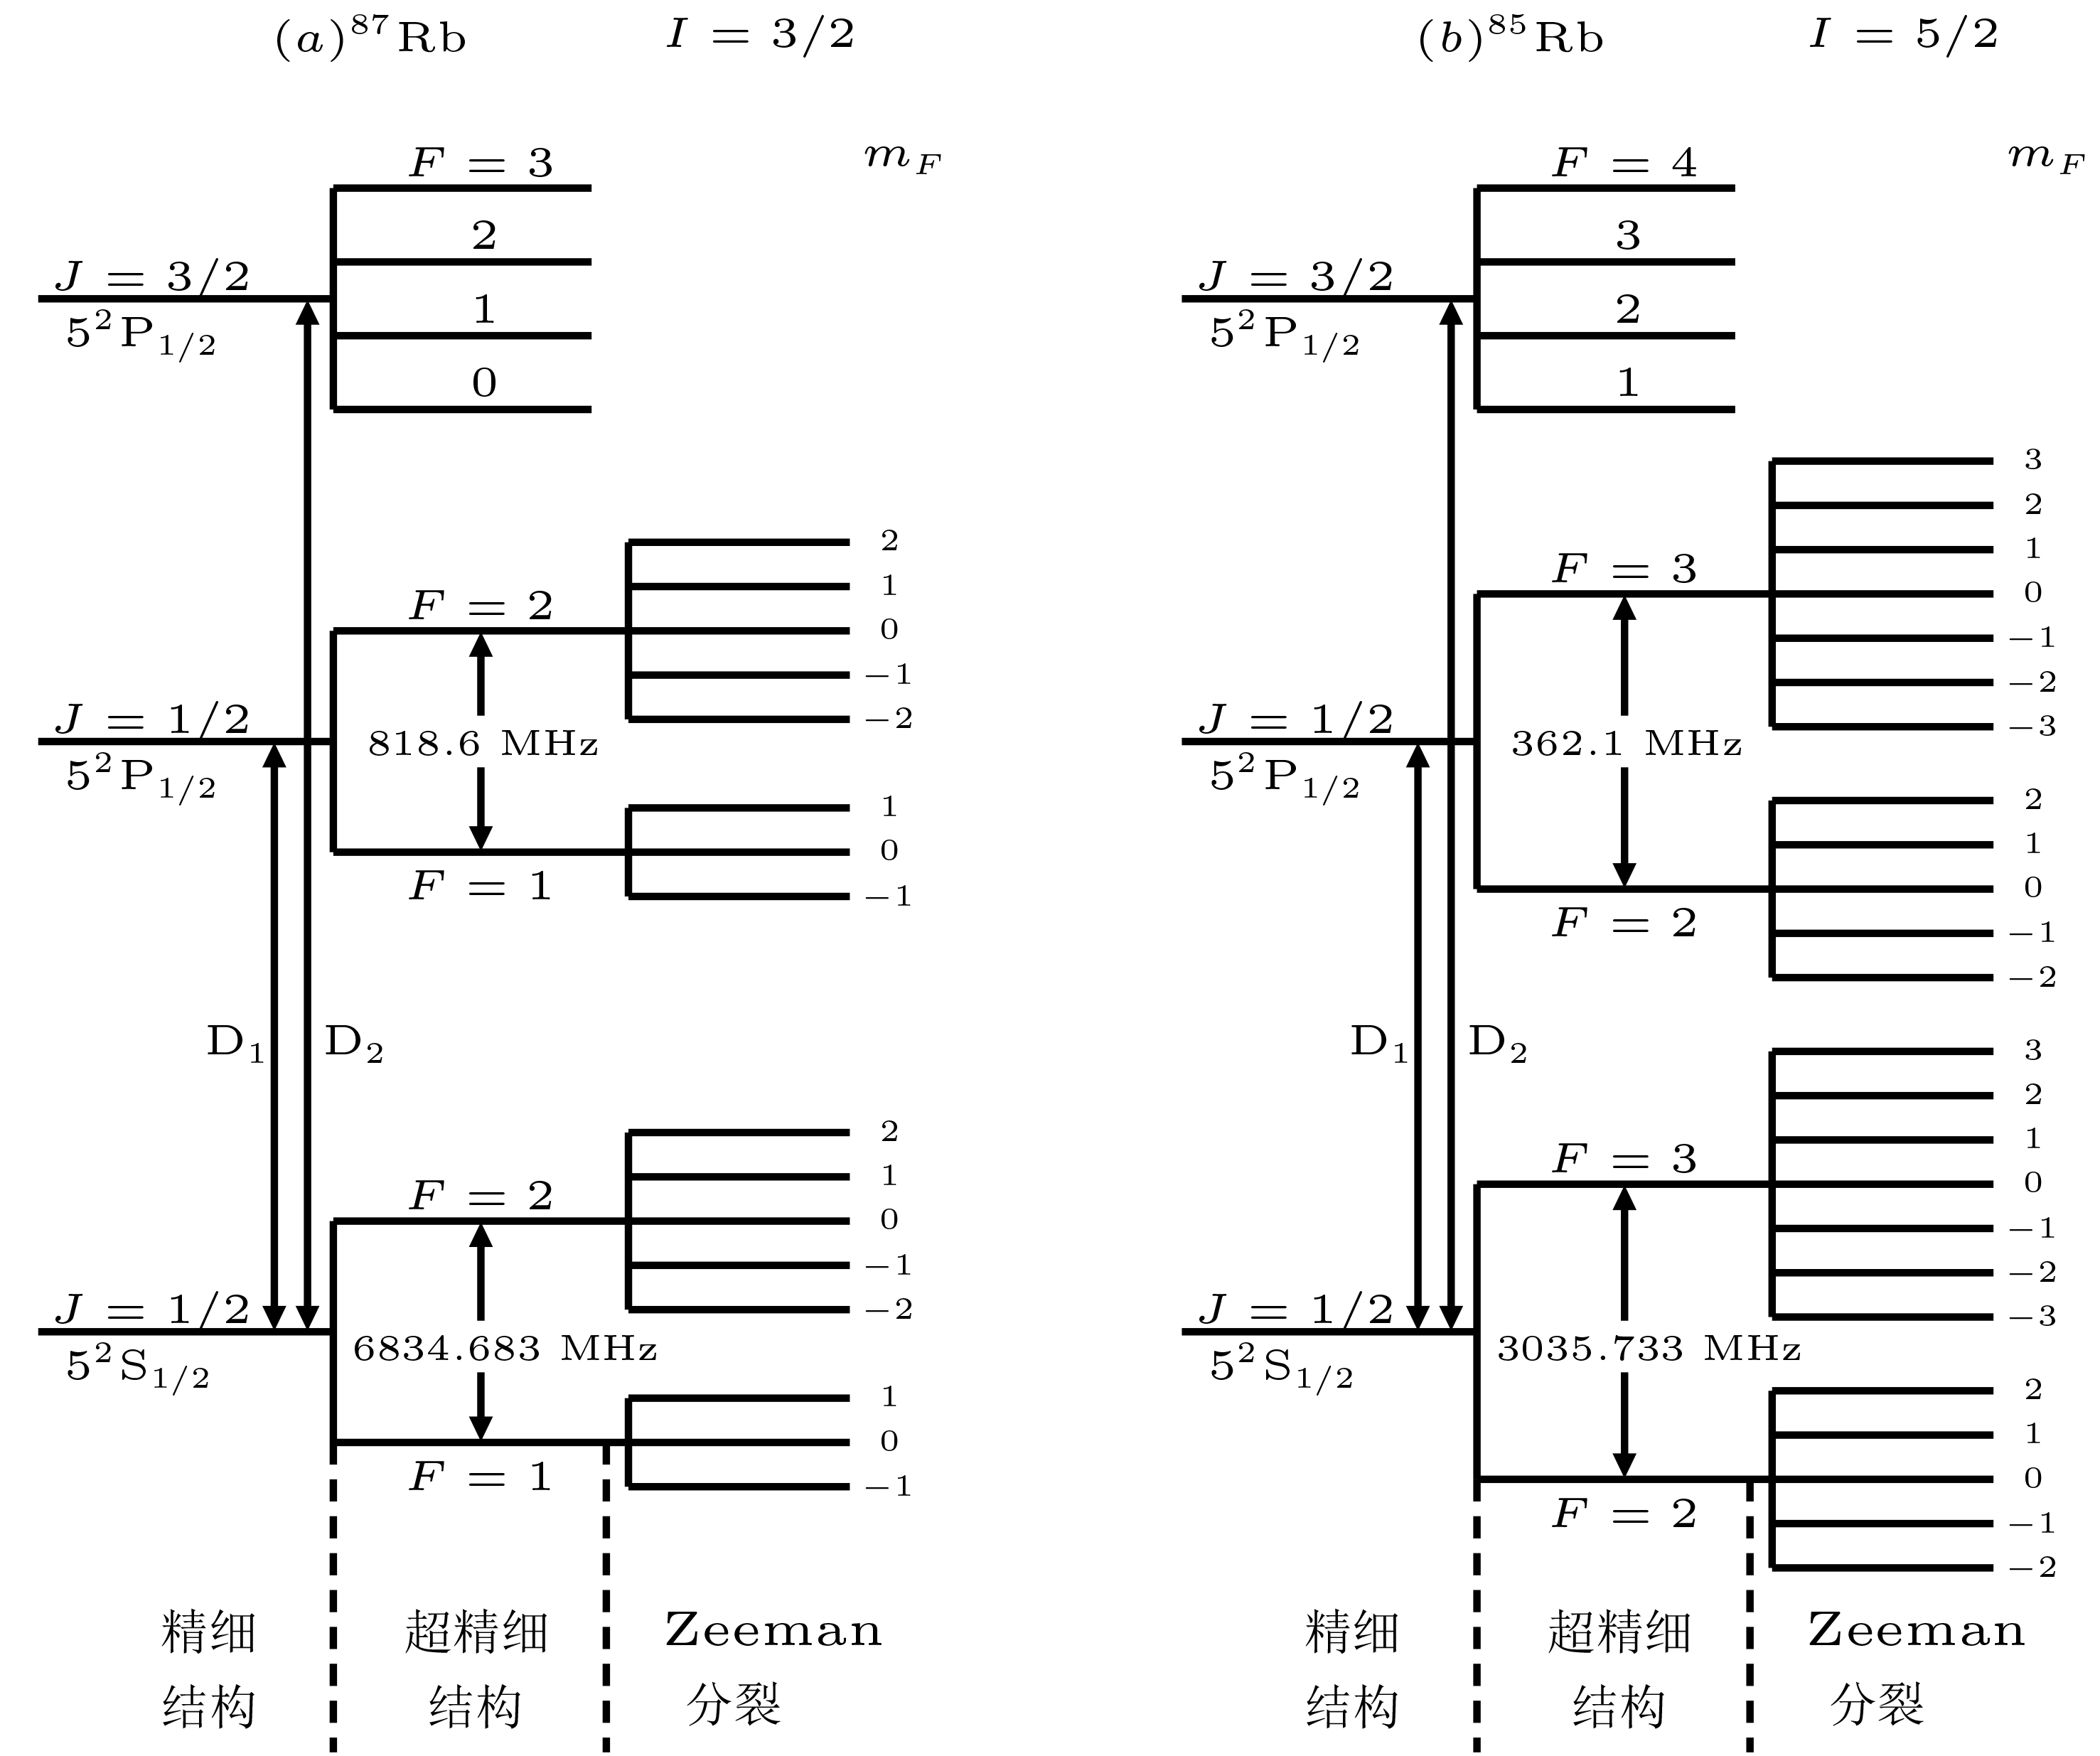
\includegraphics[width=10cm]{figures/Rbnjt.jpg}
                        \caption{铷原子能级示意图\cite{experimentBookref}}
                \end{figure}

                其中 $\mu_{B}$ 为Bohr磁子,$a$ 为磁偶极相互作用常数. 对$^{87}\mathrm{Rb}$的基态,$a_{87}=3417.34\ \mathrm{MHz}$;对$^{85}\mathrm{Rb}$的基态,$a_{85}=1011.9\ \mathrm{MHz}$.

                由(3)式可知基态 $5 ^{2}\rm S_{1/2}$ 的两个相邻超精细结构能级的能量差为:
                \begin{equation}
                        \Delta E_{F}=\frac{ah}{2}\left[F'(F'+1)-F(F+1)\right]
                \end{equation}

                由上式容易计算 $^{87}\mathrm{Rb}$ 的$\Delta E_{F}=2a_{87}h$,$^{85}\mathrm{Rb}$ 的$\Delta E_{F}=3a_{85}h$.

                同样由式\ref{eq:能级能量}还可计算相邻Zeeman子能级之间的能量差为:
                \begin{equation}\label{eq:Zeeman能级差}
                        \Delta E_{m_{F}}=g_{F}\mu_{B}B_{0}
                \end{equation}

        \subsection{磁矩和 g 因子}
        一个重要的常数是玻尔磁矩

        \begin{equation}
        \mu_{B}=\frac{\mathrm{e} \hbar}{2 m_{e}}=9.27 \times 10^{-24} \mathrm{JT}^{-1}
        \end{equation}

        电子的轨道磁矩为

        \begin{equation}
        \vec{\mu}_{L}=-\mu_{B} g_{L} \frac{\mathbf{L}}{\hbar}, g_{L}=1
        \end{equation}

        电子的自旋磁矩为

        \begin{equation}
        \vec{\mu}_{S}=-\mu_{B} g_{S} \frac{\mathbf{S}}{\hbar}, g_{S}=2.00
        \end{equation}

        考虑电子的自旋轨道耦合

        \begin{equation}
        \begin{gathered}
        \vec{\mu}=-\mu_{B} g_{J} \frac{\mathbf{J}}{\hbar} \\
        g_{J}=g_{S} \frac{j(j+1)+s(s+1)-l(l+1)}{2 j(j+1)}+g_{L} \frac{j(j+1)+l(l+1)-s(s+1)}{2 j(j+1)}
        \end{gathered}
        \end{equation}

        同理可以计算

        \begin{equation}
        g_{F}=g_{I} \frac{F(F+1)+I(I+1)-j(j+1)}{2 F(F+1)}+g_{J} \frac{F(F+1)-I(I+1)+j(j+1)}{2 F(F+1)}
        \end{equation}

        通常核自旋磁矩很小,可以忽略

        \begin{equation}
        g_{F} \approx g_{J} \frac{F(F+1)-I(I+1)+j(j+1)}{2 F(F+1)}
        \end{equation}
        铷元素在自然界有两种同位素, ${ }^{87} \mathrm{Rb}$ 占 $27.85 \%,{ }^{85} \mathrm{Rb}$ 占 $72.15 \%$ 。两种同位素的能级不一样,此外,它们的核自旋不同, $I_{85}=\frac{5}{2}, I_{87}=\frac{3}{2}$\cite{Mora_2018}。

        \subsection{光抽运效应}
                原子受到左旋偏振光 $\mathrm{D}_{1} \sigma^{+}$照射时,向上跃迁遵循的跃迁选择定则为
                \begin{equation}
                \Delta F=0, \pm 1, \Delta M_{F}=+1
                \end{equation}

                受到磁量子数的选择定则限制,处于磁量子数 $M_{F}=+2$ 的状态无法向上跃迁。因为它的跃迁状态必须是 $M_{F}=+3$ ,这个状态必须在 $F=3$ 的量子态下才存在,但是 ${ }^{87} \mathrm{Rb}$ 的 $5^{2} P_{1 / 2}$ 能级分裂的 5 量子数上限为 2 。所以无法跃迁。

                同理,受到右旋偏振光照射时,向上跃迁的选择定则为
                \begin{equation}
                \Delta F=0, \pm 1, \Delta M_{F}=-1
                \end{equation}

                选择定则会限制处于 $M_{F}=-2$ 的状态无法向上跃迁。

                若考虑向下跃迁(退激辐射),则遵循的选择定则为
                \begin{equation}
                \Delta F=0, \pm 1
                \end{equation}

                综合考虑光激发跃迁和退激的选择定则,左旋偏振光照射时原子最终都将处于 $M_{F}=+2$ 的量子态,而右旋偏振光照射时,原子都将处于 $M_{F}=-2$ 的量子态。实现了原子能级的偏极化,如图2所示。对于 ${ }^{85} \mathrm{Rb}$ ,则超精细结构量子数 $F=2,3$ ,两种偏振光的抽运过程将会使得原子能级都处于 $M_{F}=-3$ 和 $M_{F}=+3$ 的状态。
                \begin{figure}[htbp]
                        \centering
                        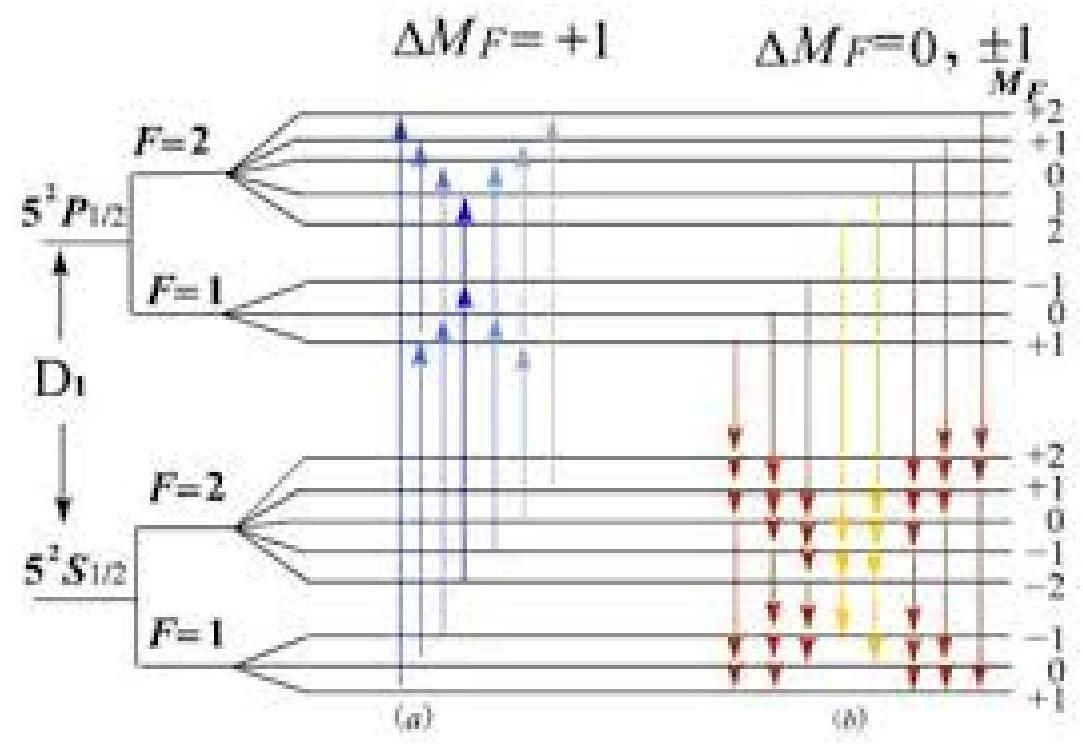
\includegraphics[width=0.5\textwidth]{figures/2024_11_21_2f14a66c261050f0bd54g-04.jpg}
                        \caption{${ }^{87} \mathrm{Rb}$ 原子光抽运过程}
                \end{figure}

                如果磁场的方向发生改变,就意味着电子的偏极化状态会发生改变,即样品泡会吸收圆偏振光。导致出射的圆偏振光变弱。光电倍增管就会在原本稳定的信号(稳定的偏极化状态会使得样品无法吸收圆偏振光)中产生向下的凹陷,这个凹陷可以通过示波器观察到,这就是抽运信号。我们将在后面的结果中观察到这个凹陷。

                顺带提及,在自然光中,各种偏振光都存在,就无法导致原子能级锁定在磁量子数的边缘。

        \subsection{磁共振}
        在垂直于产生塞曼能级分裂的磁场上增加一个交变磁场,频率为 $v$ ,当满足共振条件

        \begin{equation}
        h \nu=g_{F} \mu_{B} B 
        \end{equation}
        
        时,塞曼能级之间产生感应(磁)跃迁,遵守的选择定则为 $\Delta F=0, \Delta M_{F}= \pm 1$ 。\\
        考虑对饱和偏极化的 Rb 原子进行磁共振,不难发现磁共振会破坏偏极化分布,从而使得偏极化可以继续发生。最终光抽运和磁共振会达到一个动态平衡。光跃迁速率比磁共振跃迁速率大几个数量级,因此光抽运与磁共振的过程就可以连续地进行下去。
        
        \subsection{光探测}
                射入样品泡的$\mathrm{D}_{1}$线的$\sigma^{+}$光一方面起光抽运作用,另一方面穿过样品之后其光强的变化包含着物理性质变化的信息,所以也可以当探测光,比如发生磁共振时,
                样品对$\mathrm{D}_{1}$线的$\sigma^{+}$光吸收更多,光强也就比未磁共振时更小,所以测量透过样品后的光强变化则可以得到磁共振相关的信号,从而实现对磁共振的光探测. 

                所以利用光泵磁共振技术可以将对一个低频射频光子($1-10\ \mathrm{MHz}$)的探测转换成对一个高频光频光子($10^{8}\ \mathrm{MHz}$)的探测,使得对信号的探测灵敏度提高了七到八个数量级.

\section{实验过程}
        \subsection{实验仪器介绍}
                本实验采用的Rb原子光泵磁共振实验装置如图\ref{fig:实验装置}所示. 
                \begin{figure}[htbp]\label{fig:实验装置}
                        \centering
                        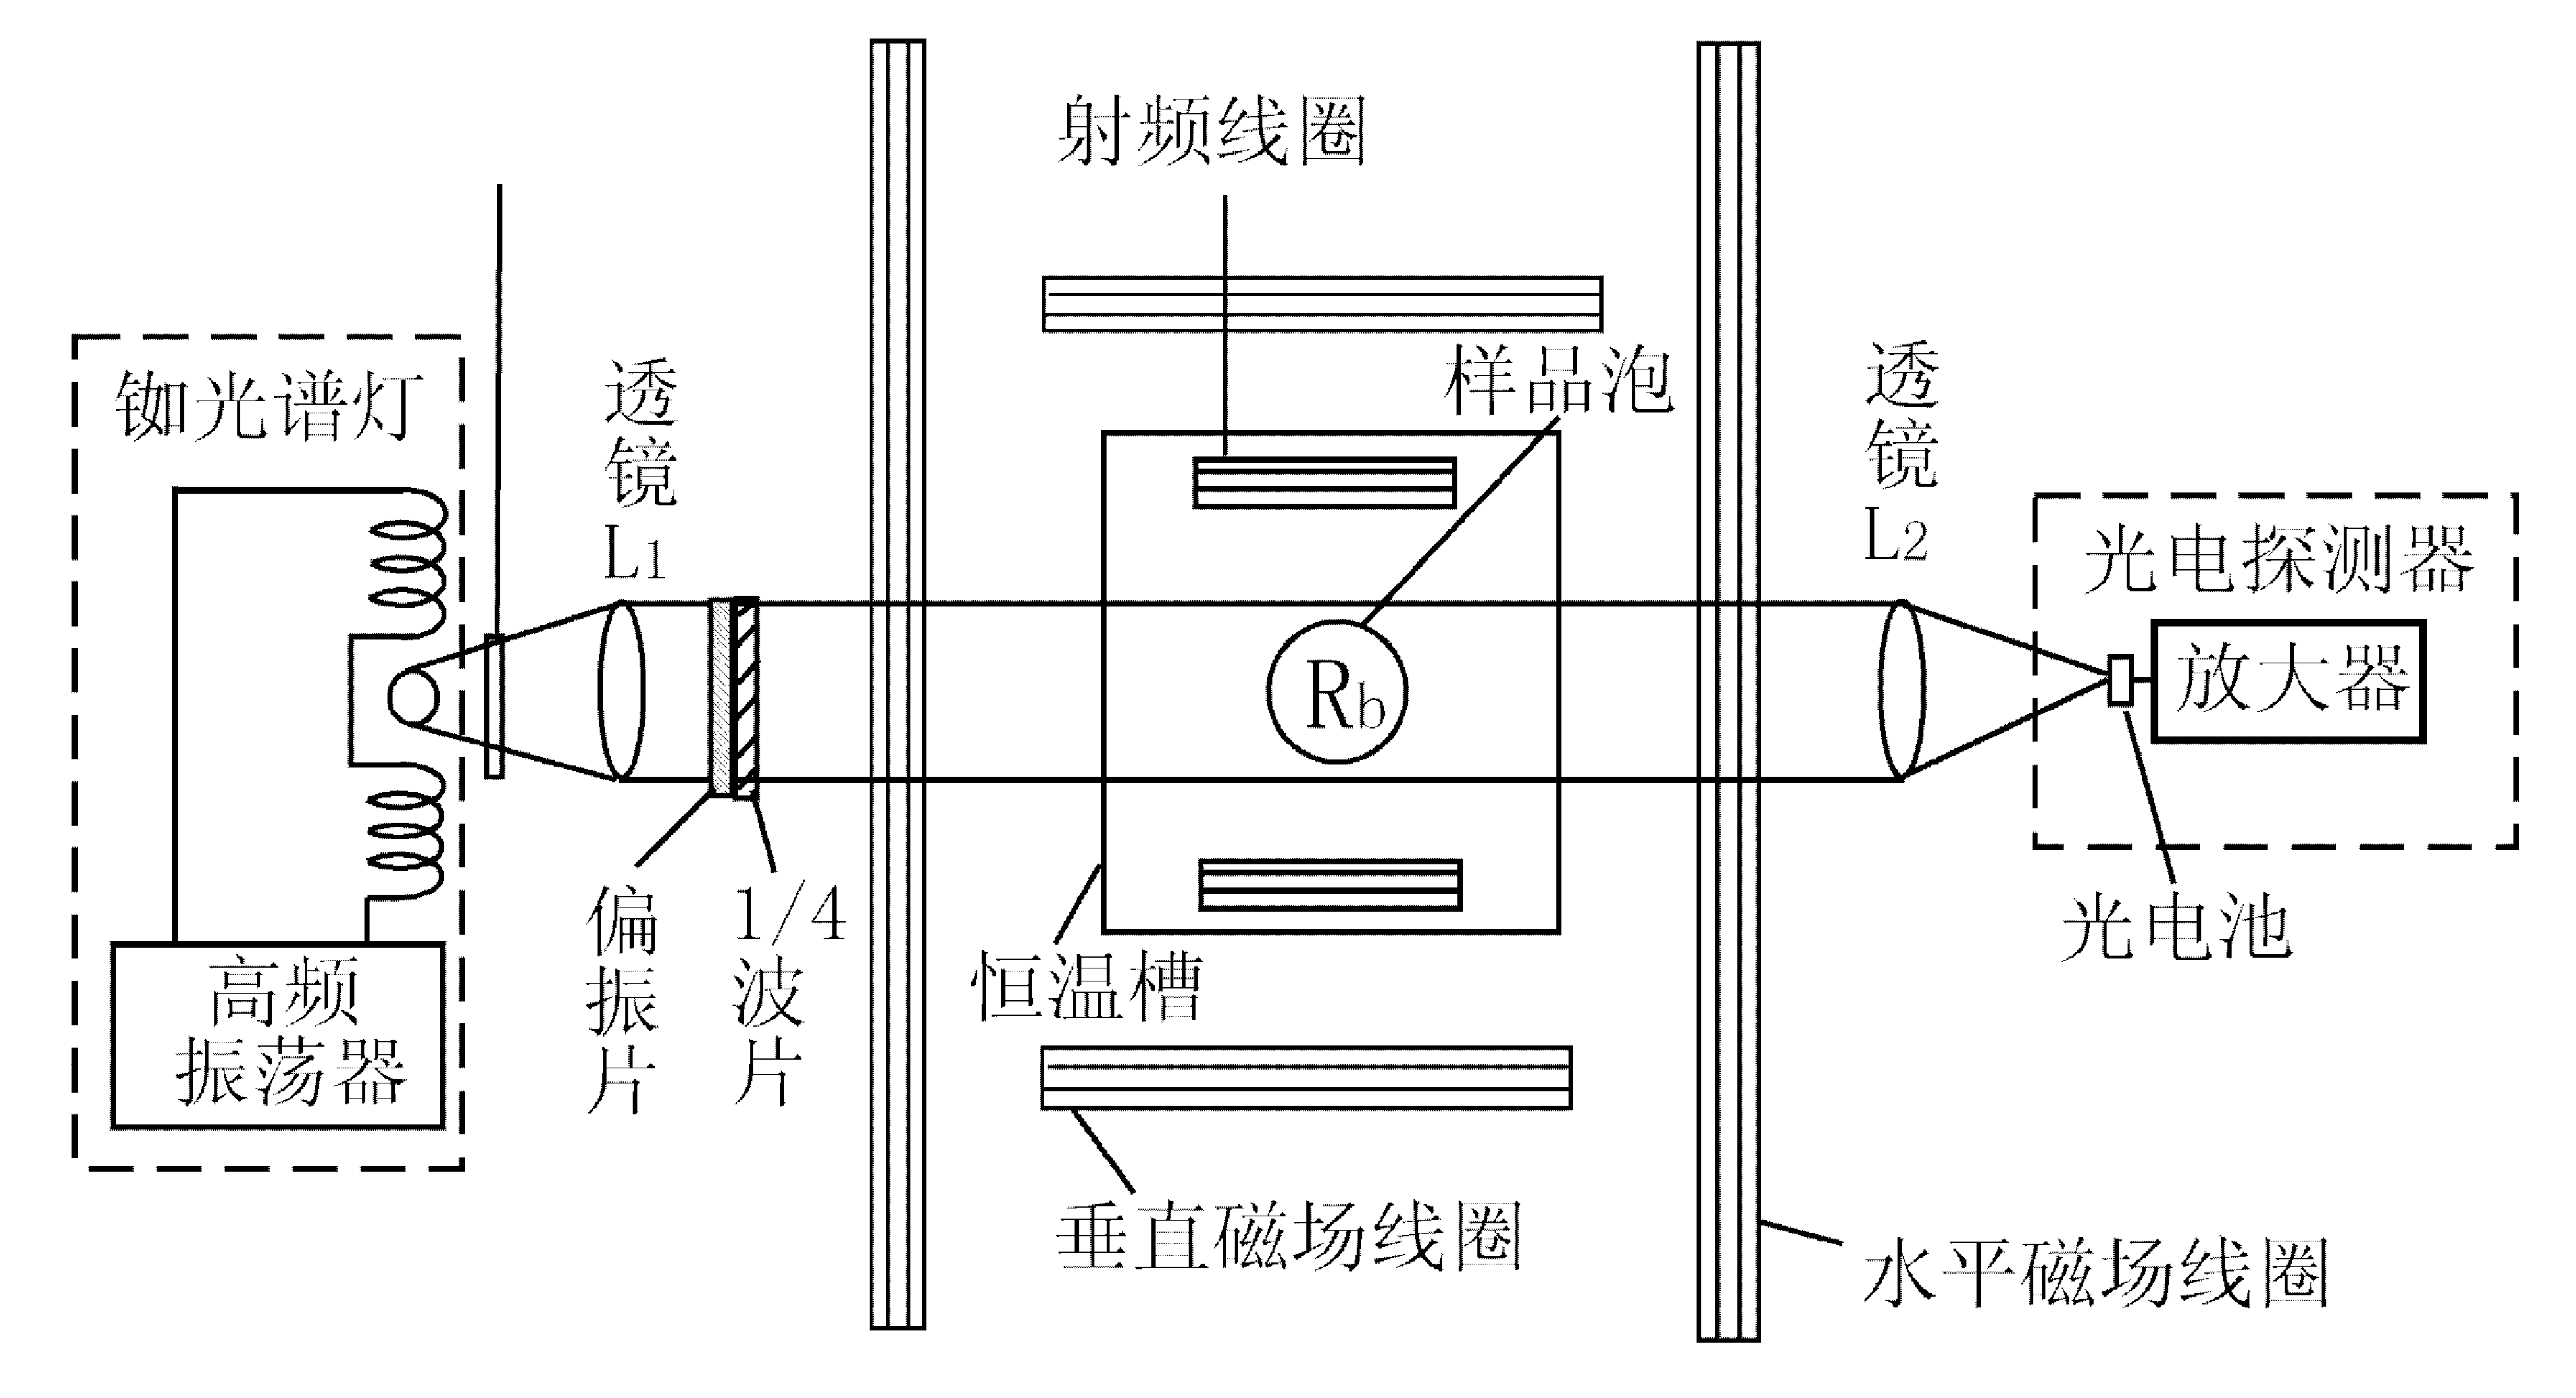
\includegraphics[width=10cm]{figures/syzz.jpg}
                        \caption{光泵磁共振实验装置示意图\cite{2007近代物理实验}}
                \end{figure}

                主体中央为铷样品泡及磁场线圈部分。同位素比例为天然成分的铝和缓冲气体充在一直径为 $52 \unit{\centi\meter}$ 的玻璃泡内。这里一共有四组线圈,分别产生射频场、水平磁场、水平扫场和坚直磁场。

                \begin{itemize}
                  \item 在铷样品泡的前后两侧对称放置一对小射频线圈,它为铷原子磁共振跃迁提供射频场。铷样品泡和射频线圈都置于圆柱形恒温槽内,称之为吸收池。槽内温度控制在最佳范围内温度。吸收池安放在两对亥姆霍兹线圈的中心。
                  \item 一对竖直线圈产生的磁场用以抵消地磁场的竖直分量。
                  \item 水平线圈有两套绕组,一组在外,为产生水平直流磁场的线圈。水平直流磁场是调节磁场的基础,使铷原子的超精细结构能级发生塞曼分裂的是水平方向的总磁场。
                  \item 水平线圈有两套绕组,另一组在内,为扫场线圈,扫场是在直流磁场上叠加的一个调制磁场(方波或三角波),值得注意的是,叠加上去的这个磁场始终是单极性的,即扫场扫面过程中的方向不会改变,在 0 和某个值之间来回变化。
                \end{itemize}

        \subsection{主要实验内容}
        \begin{itemize}
                \item[1)] 加热样品泡和 Rb 灯:将样品泡温度稳定在 $40^{\circ}\mathrm{C}-60^{\circ}\mathrm{C}$,Rb 灯温度约 $90^{\circ}\mathrm{C}$。预热约半小时,待“灯温”和“池温”指示灯亮后开始实验。
                \item[2)] 调节光路:调整光源、透镜、样品泡和光电池的位置,使入射光平行,并调节 $\rm L_{2}$ 以最大化光电池受光量,获得最佳信号。
                \item[3)] 消除地磁场垂直分量:将扫场线圈输出设为方波,调节振幅使磁场为 $0.5-1\ \rm Gs$。通过调整垂直磁场线圈,抵消地磁场垂直分量,以增强光抽运信号。观察光强的动态变化过程,确保信号最佳。
                \item[4)] 测量磁共振信号:采用扫场法固定射频场频率,调节恒定磁场大小,记录 $^{87}\mathrm{Rb}$ 和 $^{85}\mathrm{Rb}$ 的磁共振磁场值。计算基态超精细结构朗德因子 $g_{F}$ 和地磁场大小,并与理论值比较。
        \end{itemize}

\section{实验结果和分析}
        \subsection{光抽运信号的观察}
                调节通过水平和垂直亥姆霍兹线圈的电流,以补偿地磁场,我们也可以通过这一步计算地磁场的矢量值;首先使用如下式\ref{eq:场强计算}计算:
                        \begin{equation}\label{eq:场强计算}
                                B_{\mbox{\scriptsize 水平场}}=\frac{16\pi}{5^{3/2}}\times\frac{N}{r}\times I\times 10^{-3};\\
                                B_{\mbox{\scriptsize 垂直场}}=\frac{32\pi}{5^{3/2}}\times\frac{N}{r}\times I\times 10^{-3}
                        \end{equation}

                其中:$N$为线圈每边匝数;$r(\unit{\meter})$为线圈有效半径,$I(\unit{\milli A})$为流过线圈电流;磁感应强度$B(\unit{Gs})$. 水平场线圈并联,垂直场线圈串联,因此水平场线圈电流实际上为度数的$1/2$。
                                        
                本实验中用到的不同的亥姆霍兹线圈的参数如表\ref{tab:线圈参数}所示:
                        \begin{table}[H]\label{tab:线圈参数}
                                \caption{\textbf{不同线圈参数}}
                                \setlength{\tabcolsep}{0.6cm}
                                \centering
                                \begin{tabular}{|c|c|c|c|}
                                        \hline
                                        &线圈匝数&有效半径$(\unit{\meter})$ & 电阻$(\unit{\ohm})$\\ \hline
                                        水平场线圈& 250 & $0.2393$ & 24.14 \\ \hline
                                        扫场线圈  & 250 & $0.2360$ & 24.68\\ \hline
                                        垂直场线圈& 100 & $0.1530$ & 23.71\\ \hline
                                \end{tabular}
                        \end{table}

                总磁场则有以下式\ref{eq:总磁场}计算:
                        \begin{equation}\label{eq:总磁场}
                                \vec{B}=\vec{B}_{\mbox{\scriptsize 水平场}}+\vec{B}_{\mbox{\scriptsize 垂直场}}+\vec{B}_{\mbox{\scriptsize 扫场}}+\vec{B}_{\mbox{\scriptsize 地磁场}}
                        \end{equation}

                调整扫场方式为方波并调整为与地磁场同向,并且将水平场调节为与地磁场反向。调节水平场和扫场幅度,能观察到明显的光抽运现象,如图\ref{fig:光抽运信号}:
                        \begin{figure}[htbp]\label{fig:光抽运信号}
                                \centering
                                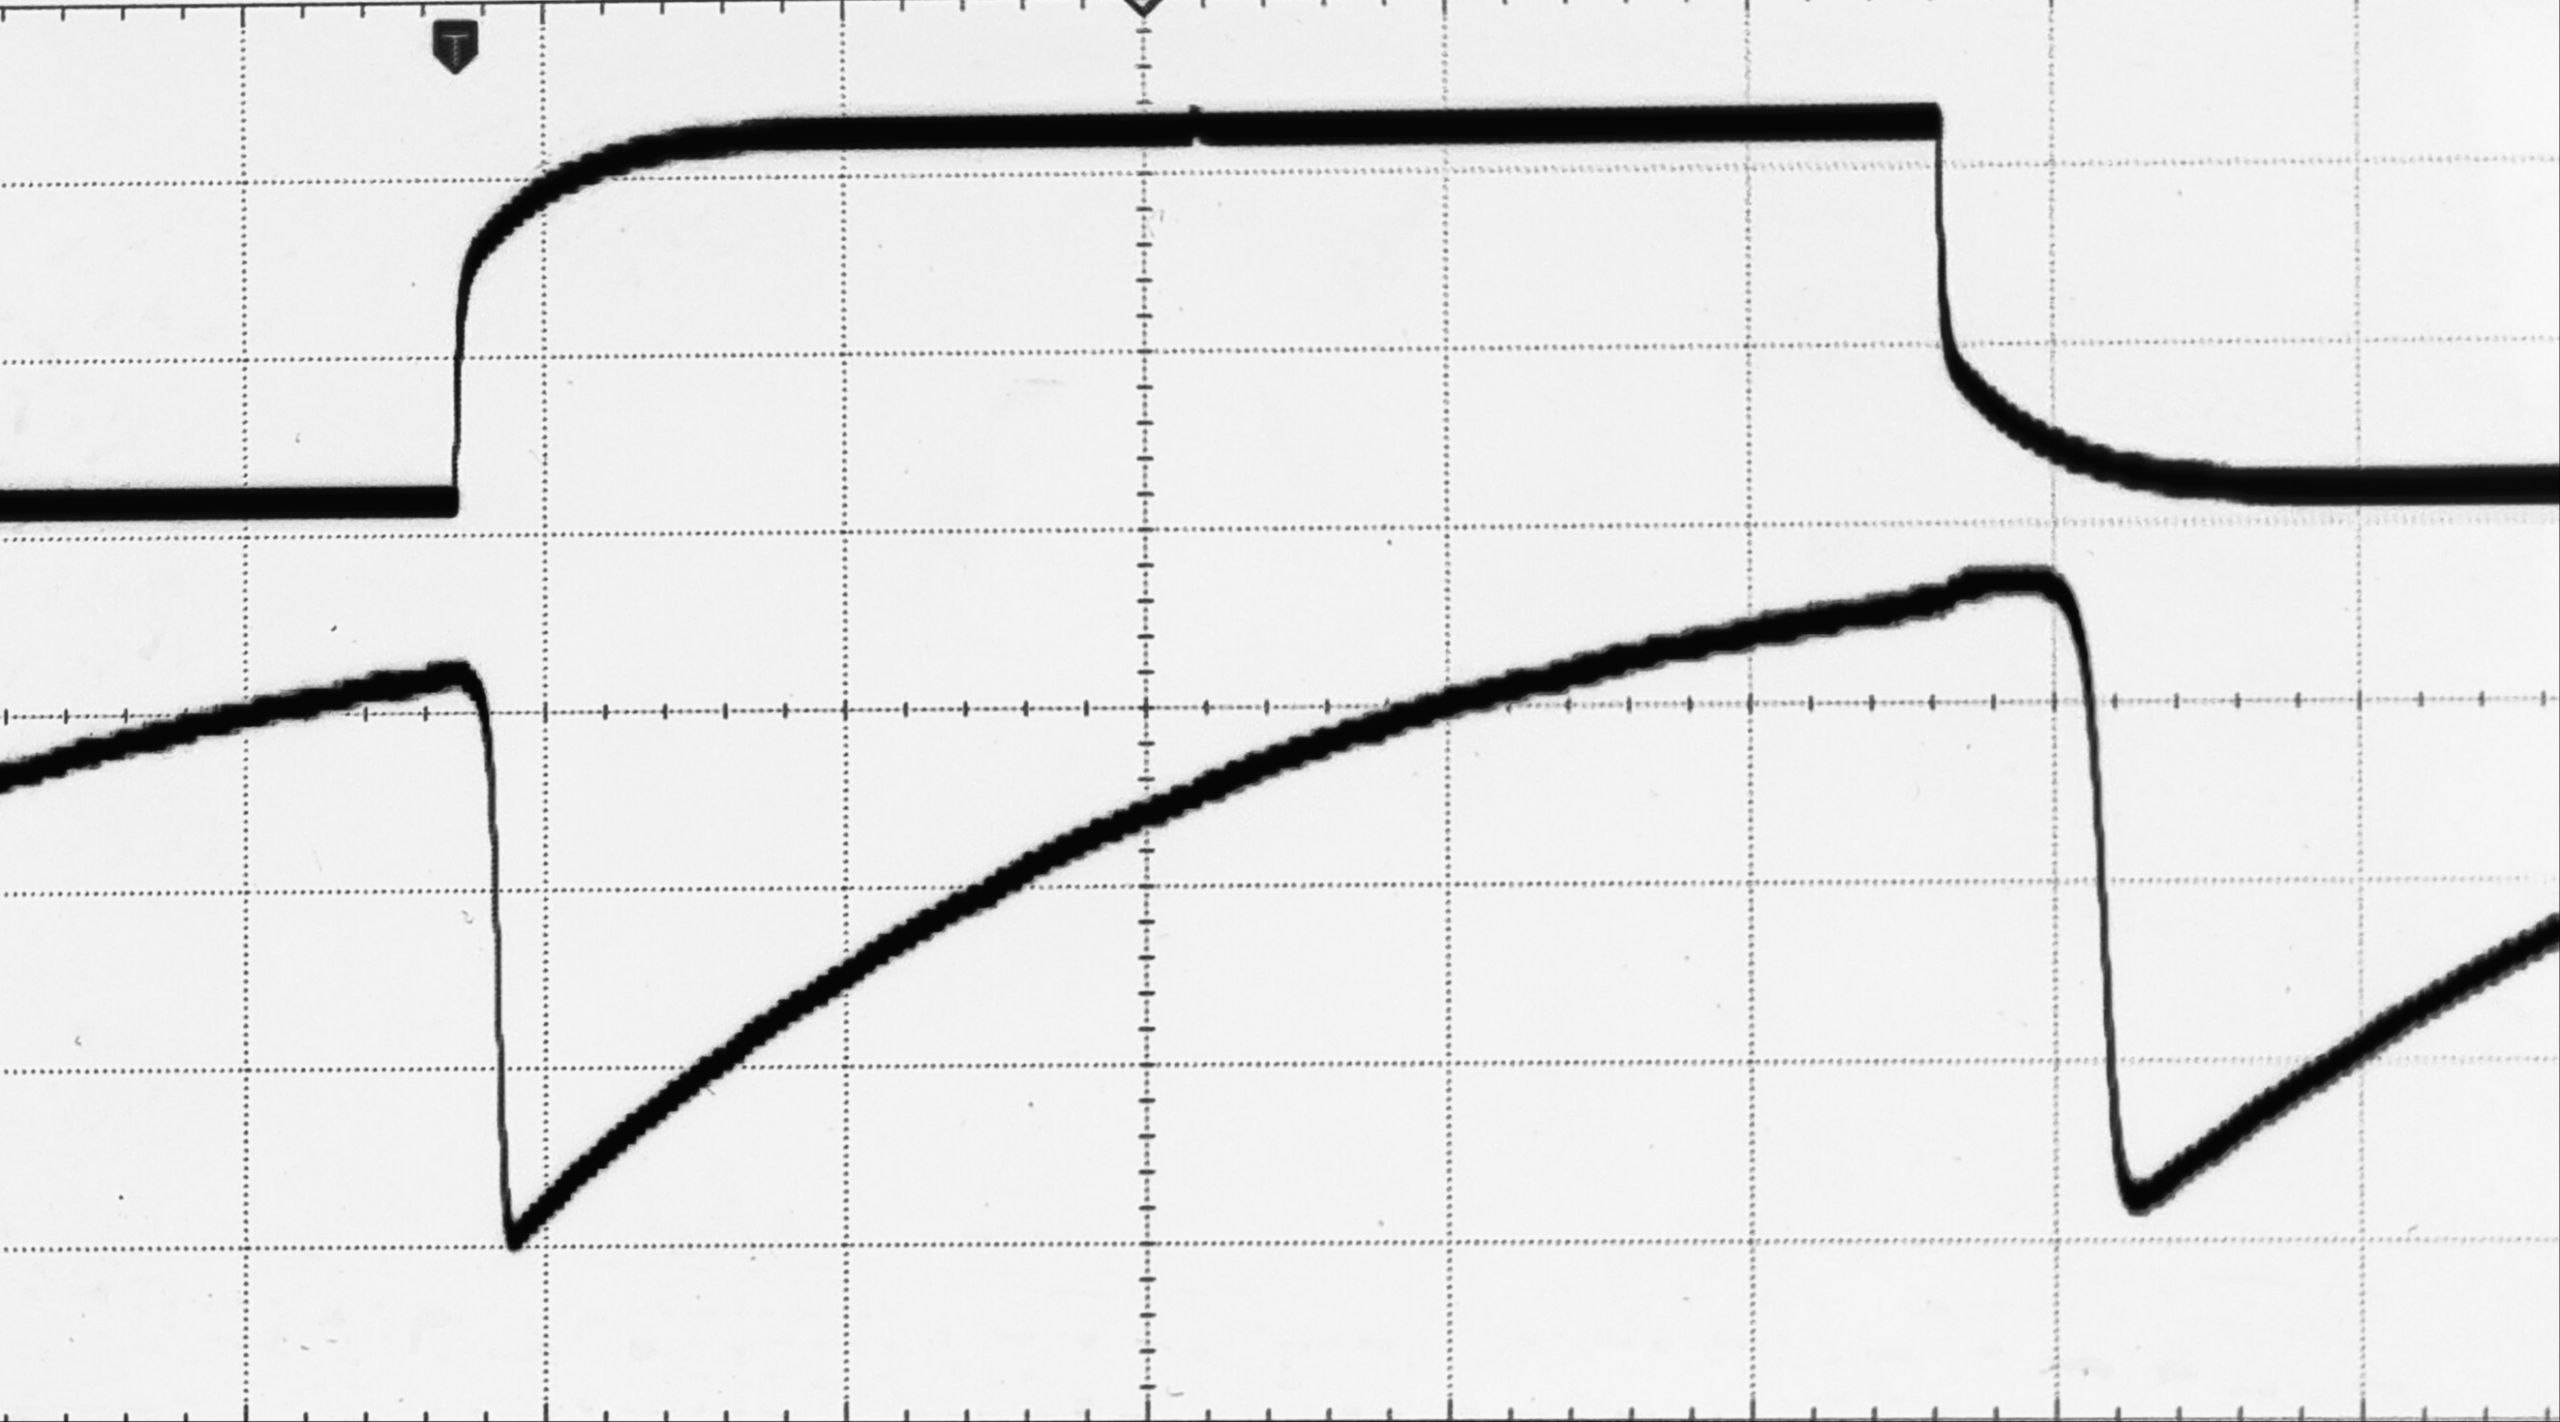
\includegraphics[width=8cm]{figures/IMAGE 2024-11-22 01:28:39.jpg}
                                \caption{光抽运信号图}
                        \end{figure}

                设置垂直场方向与地磁场反向,调节垂直场大小,使得光抽运现象最明显,说明此时扫场信号使得总磁场过零,即可以认为垂直磁场抵消地磁场,记录此时通过垂直磁场线圈的电流:
                $$
                        I_{\perp}=0.064 \sim 0.074\unit{A} ;\quad \bar{I_{\perp}}=0.069\unit{A}
                $$

                根据式\ref{eq:场强计算}可以计算出地磁场垂直方向分量:
                        \begin{equation*}
                        B_{\perp}=\frac{32\pi}{5^{3/2}}\frac{NI}{r}\times 10^{-3}=0.436\unit{Gs}
                        \end{equation*}

                之后实验中均保持垂直方向磁场不变,以获得最佳光信号. 

                另一方面,最开始观察到的光抽运信号图(图\ref{fig:光抽运信号}),在方波的一个周期内,前半个周期的光信号和后半个周期光信号的波形并不一致. 此时两方向总场强度不同,调整水平磁场使得两个周期内的光信号波形一致,如图\ref{fig:光抽运信号(平衡)}所示. 记录此时通过水平磁场线圈的电流大小:
                        \begin{figure}[htbp]\label{fig:光抽运信号(平衡)}
                                \centering
                                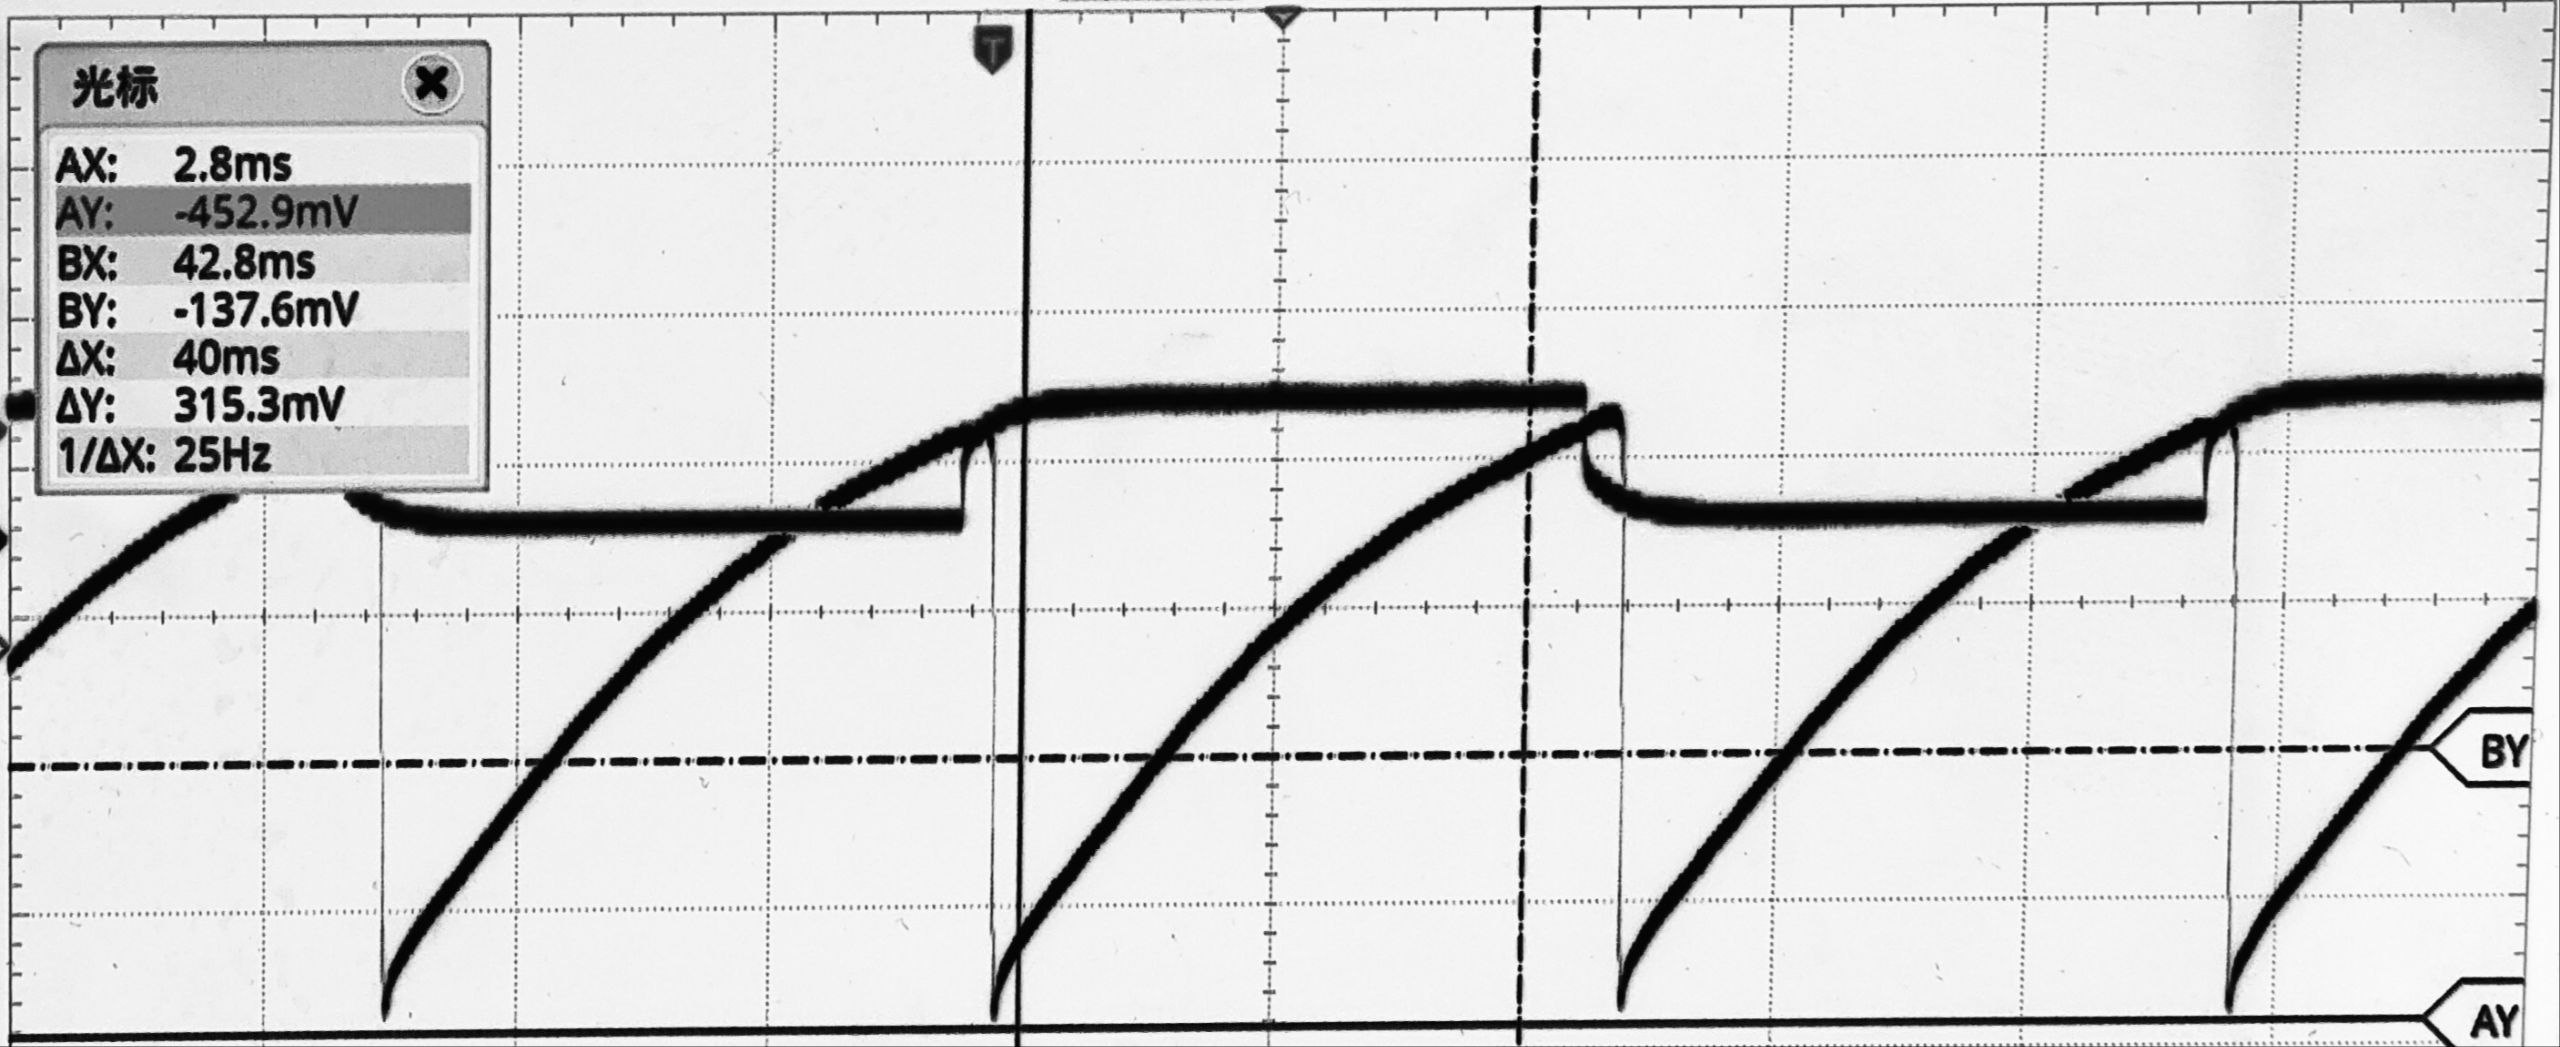
\includegraphics[width=8cm]{figures/IMAGE 2024-11-22 01:28:40.jpg}
                                \caption{光抽运信号图(平衡)}
                        \end{figure}

                记录此时通过水平磁场线圈的电流大小:
                        $$I_{-}=0.125\unit{A}$$

                设加入的扫场的平均值为$\bar{B}_{scan}$,地磁场平行方向分量为$B_{geo\pll}$,此时水平场大小为$B_{\pll +}$

                根据上面的分析可以得到方程:
                        \begin{equation}\label{eq:地磁场平行方向分量1}
                                B_{\pll}=\bar{B}_{scan}-B_{\pll +}
                        \end{equation}

                将水平和扫描场同时反向,并再次调节水平场大小使得波形图达到类似图\ref{fig:光抽运信号(平衡)},并记录此时通过水平磁场线圈的电流大小:
                        \begin{equation*}
                                I_{2}=0.254\ \rm A
                        \end{equation*}

                设此时水平场大小为$B_{\pll -}$,则可得到方程:
                        \begin{equation}\label{eq:地磁场平行方向分量2}
                                B_{\pll}=-\bar{B}_{scan}+B_{\pll -}
                        \end{equation}

                由式\ref{eq:场强计算},\ref{eq:地磁场平行方向分量1},\ref{eq:地磁场平行方向分量2}可以计算出地磁场水平方向分量:
                        \begin{equation*}
                        \begin{split}
                        B_{\pll}&=\frac{1}{2}\left(B_{\pll 1}+B_{\pll 2}\right) \\
                        &=\frac{8\pi}{5^{3/2}}\frac{N(I_{2} - I_{1})}{r}\times\ 10^{-3} \\
                        &=0.302\ \unit{Gs}
                        \end{split}
                        \end{equation*}

        \subsection{磁共振信号的观察}
                在磁共振实验中,加入频率$f=650\ \rm kHz$的射频场,并调节扫场输出信号为三角波. 
                使用不同的扫场,加入或不加入坚直线圈磁场及水平线圈磁场,以及改变它们的励磁电流大小和方向都将影响光抽运信号。
                        \begin{figure}[htbp]\label{fig:磁共振信号磁场}
                                \centering
                                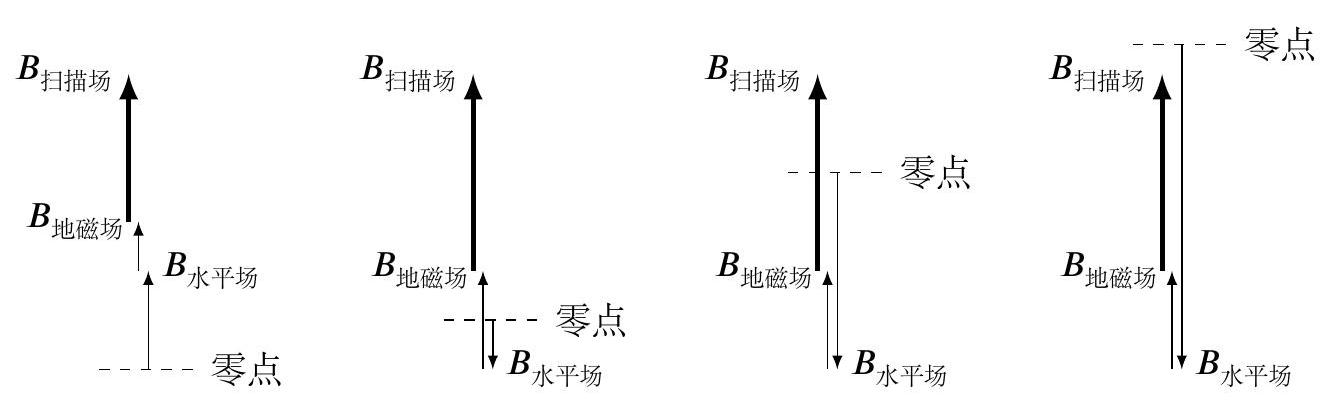
\includegraphics[width=\textwidth]{figures/2024_11_21_2f14a66c261050f0bd54g-08.jpg}
                                \caption{磁场方向关系和抽运信号产生:扫描场是在 0 和给定幅度之间扫描,故将其加粗,水平场的调节通过调节电路中电流大小实现。根据抽运信号发生的机制,如果扫描场导致磁场方向改变(过零)就会产生抽运信号}
                        \end{figure}


                \noindent
                在调节过程中,我们固定使用三角波信号幅度,调节水平场大小和方向使得在某一时刻总磁场大小等于$B_{0}$,此时观察到磁共振信号.考虑到三角波扫描有上升沿和下降沿,因此一般在一个周期内可能会出现两次磁共振信号,但当磁场强度极大值和极小值正好为$B_{0}$时,只会出现一次磁共振信号。此时,我们可以说:

                \begin{equation}\label{eq:磁共振条件}
                        B_{geo\pll} \pm B_{\pll} \pm B_{scan\ min/max} = \pm B_0
                \end{equation}

                同时,我们考虑扫描场强度较小,即:$B_{scan\ max} < B_0$的情况。

                其中正负号取决于扫场和水平场方向,与地磁场同向为正,反向为负。并且当$B_{\pll}$前符号取负时,公式\ref{eq:磁共振条件}右侧绝对值符号内部分为负,此时有:$B_{geo\pll} - B_{\pll} \pm B_{scan\ min/max} = -B_0$,同时,扫描场前符号取决于达到扫场的方向, min/max与核磁共振信号是在扫场信号峰处出现还是谷处出现相关。

                这里以情况$(+,+)$与$(+,-)$描述发生的情况:
                \begin{itemize}
                        \item[1)] $I_{\pll}$在初始时为 0,此时总场在$B_{geo\pll}+B_{scan\ min} \sim B_{geo\pll}+B_{scan\ max} $间扫描,且总场始终小于$B^{87}_0$,因此不会发生磁共振现象.如图\ref{fig:情况1},信号为一条直线.
                        \item[2)] $I_{\pll}$逐渐增大,当$I_{++1}=0.075\ \rm A$时,总场最大值等于$B^{87}_{0}$,此时发生磁共振现象.如图\ref{fig:情况2},高信号基底上出现陡降的缺口,时间与扫场信号达峰时一致,该信号表明一个周期内发生且只发生一次磁共振,满足公式:$B_{geo\pll} + B_{\pll} + B_{scan\ max} = B^{87}_0$.
                        \item[3)] 继续增大,在一个周期中,核磁共振信号出现两次,如图\ref{fig:情况3},此时$B_{geo\pll} + B_{\pll} + B_{scan\ max} > B^{87}_0$,$B_{geo\pll} + B_{\pll} + B_{scan\ min} < B^{87}_0$,因此在扫描过程中,总场两次达到$B_0$,因此发生两次磁共振.
                        \item[4)] 继续增大,当$I_{++2}=0.126\ \rm A$时,总场最小值等于$B^{87}_{0}$,此时发生磁共振现象.如图\ref{f},信号与情况2类似,但信号波形相反,此时$B_{geo\pll} + B_{\pll} + B_{scan min} = B^{87}_0$.
                        \item[5)] 继续增大,在一段增量内,总场始终大于$B^87_0$,不会发生磁共振现象,信号为一条直线.
                        \item[6)] 继续增大,当$I_{++3}=0.173\ \rm A$时,总场最大值等于$B^{85}_{0}$,此时发生磁共振现象,信号与情况2类似,此时$B_{geo\pll} + B_{\pll} + B_{scan\ max} = B^{85}_0$. 
                        \item[7)] 继续增大,发生同上 3),4)情况,这是由于我们此时与$Rb^{85}$发生核磁共振,记第四次共振电流为:$I_{++4}$.
                \end{itemize}

                \begin{figure}[htbp]
                        \centering
                        
                        \subfigure[情况 1]{
                        \begin{minipage}[t]{0.25\linewidth}
                        \centering
                        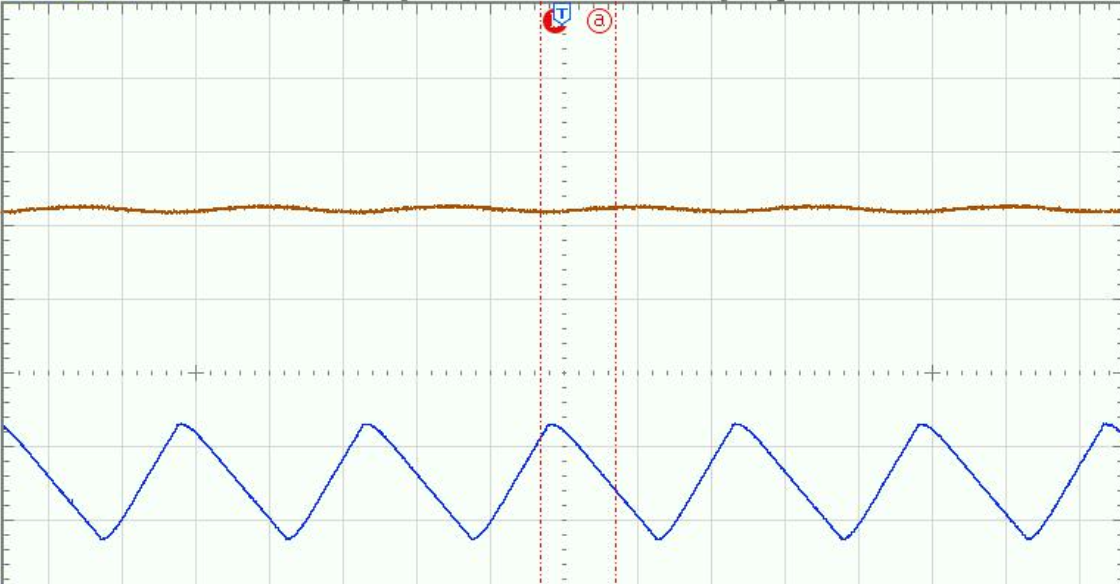
\includegraphics[width=1in]{figures/figure0.png}
                        %\caption{fig1}
                        \end{minipage}%
                        }\label{fig:情况1}
                        \subfigure[情况 2]{
                        \begin{minipage}[t]{0.25\linewidth}
                        \centering
                        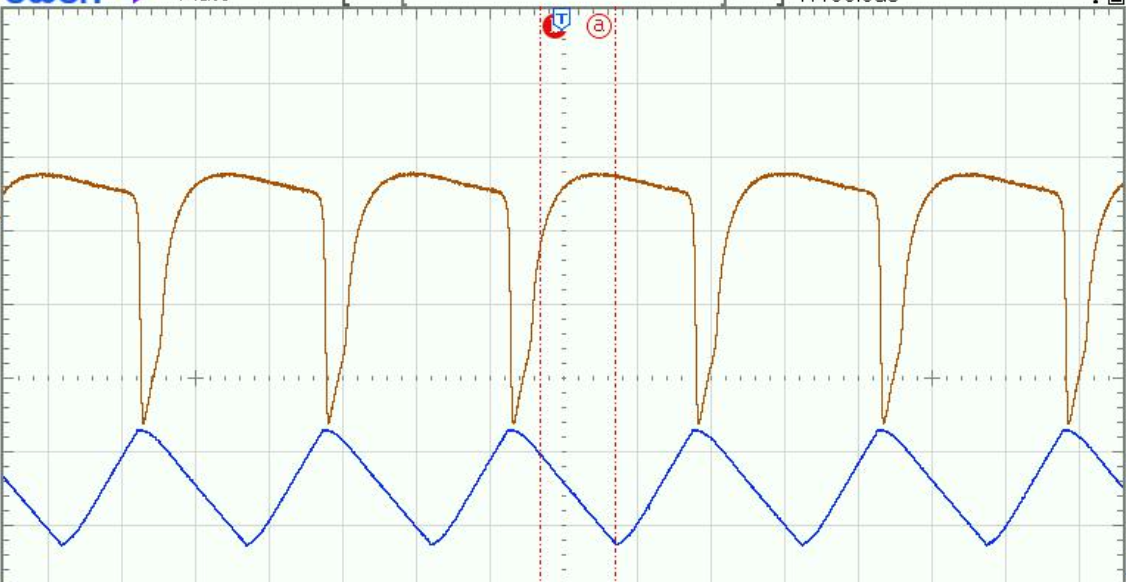
\includegraphics[width=1in]{figures/figure1.png}
                        %\caption{fig2}
                        \end{minipage}%
                        }\label{fig:情况2}
                        
                        \subfigure[情况 3]{
                        \begin{minipage}[t]{0.25\linewidth}
                        \centering
                        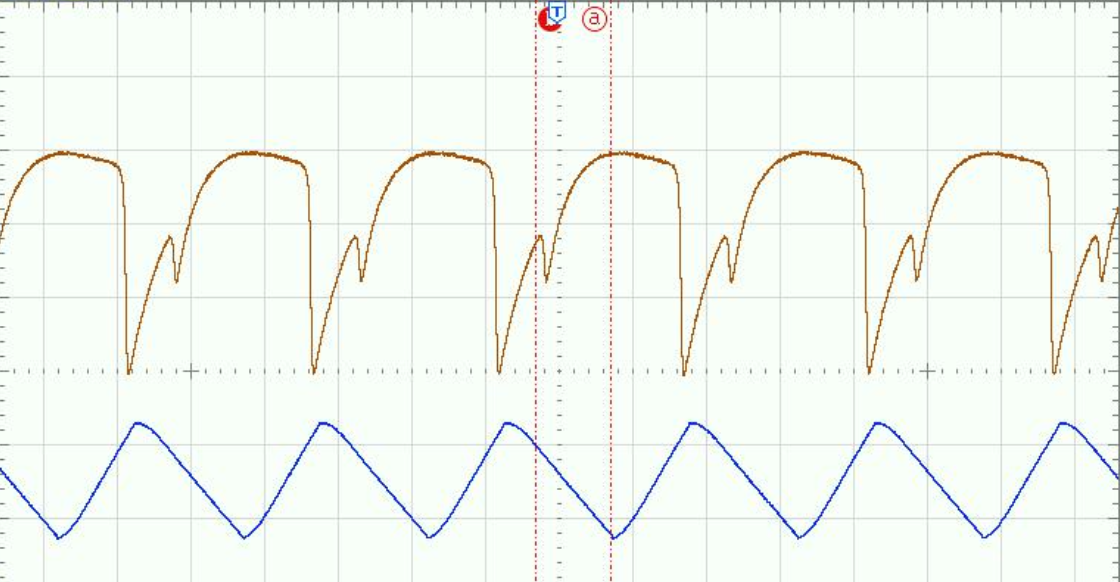
\includegraphics[width=1in]{figures/figure2.png}
                        %\caption{fig2}
                        \end{minipage}
                        }\label{fig:情况3}
                        \subfigure[情况 4]{
                        \begin{minipage}[t]{0.25\linewidth}
                        \centering
                        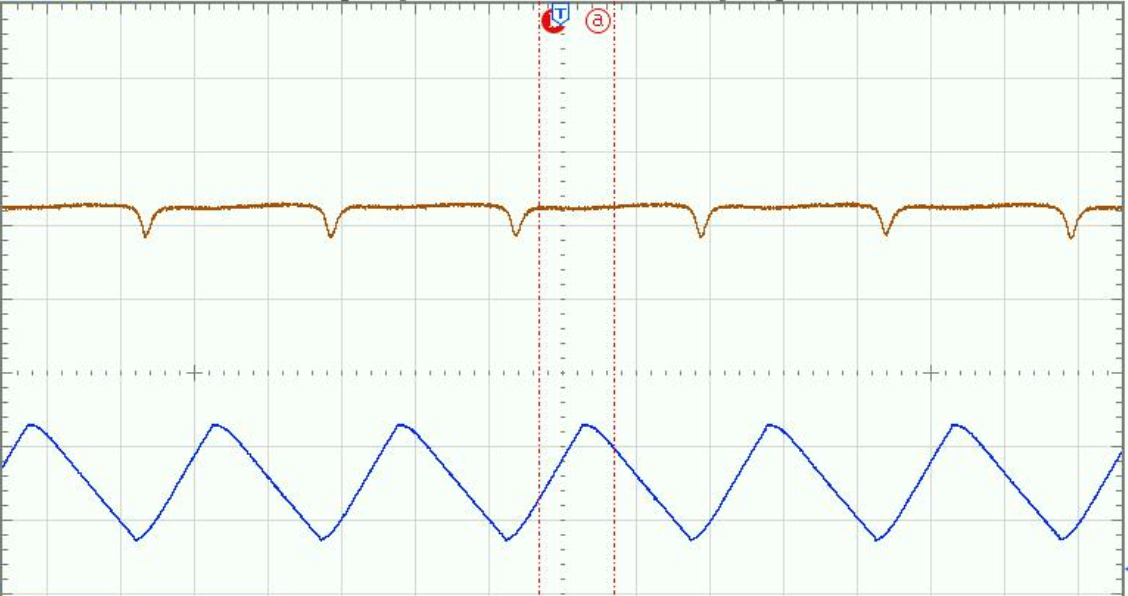
\includegraphics[width=1in]{figures/figure3.png}
                        %\caption{fig2}
                        \end{minipage}
                        }\label{fig:情况4}
                        
                        \centering
                        \caption{磁共振信号波形图}
                \end{figure}

                通过多次调节扫场和水平场方向,并测量达到核磁共振的电流,我们整理出如下表格:
                
                \begin{table}[htbp]
                        \caption{\textbf{磁共振临界情况电流大小}}
                        \setlength{\tabcolsep}{0.6cm}
                        \centering
                        \begin{tabular}{cccccc}
                        \toprule
                        扫场&水平场&1&2&3&4 \\
                        \midrule
                        $+$&$+$& 0.075 A & 0.126 A & 0.173 A & 0.224 A \\
                        $+$&$-$& 0.271 A & 0.323 A & 0.370 A & 0.421 A \\
                        $-$&$+$& 0.163 A & 0.213 A & 0.261 A & 0.311 A \\
                        $-$&$-$& 0.185 A & 0.235 A & 0.283 A & 0.333 A \\
                        \bottomrule
                        \end{tabular}
                \end{table}\label{tab:磁共振临界情况电流大小}

        同时由磁场的线性叠加性,我们可以直接利用式\ref{eq:场强计算}计算出各个部分的磁场大小,如表\ref{tab:磁场大小}所示:
                \begin{table}[htbp]
                        \caption{\textbf{磁场大小}}
                        \setlength{\tabcolsep}{0.6cm}
                        \centering
                        \begin{tabular}{cccccc}
                        \toprule
                        扫场&水平场&1&2&3&4 \\
                        \midrule
                        $+$&$+$& 0.352 Gs & 0.592 Gs & 0.816 Gs & 1.08 Gs \\
                        $+$&$-$& 1.272 Gs & 1.512 Gs & 1.736 Gs & 1.976 Gs \\
                        $-$&$+$& 0.768 Gs & 1.000 Gs & 1.224 Gs & 1.464 Gs \\
                        $-$&$-$& 0.872 Gs & 1.104 Gs & 1.328 Gs & 1.560 Gs \\                \bottomrule
                        \end{tabular}
                \end{table}\label{tab:磁场大小}
                这个表中各个位置对应公式\ref{eq:磁共振条件}中的$B_{\pll}$,$B_{scan\ min/max}$,$B_{0}$的正负情况如下表\ref{tab:磁场符号}所示:

                \begin{table}[htbp]
                        \caption{\textbf{磁场符号}}
                        \setlength{\tabcolsep}{0.6cm}
                        \centering
                        \begin{tabular}{cccccc}
                        \toprule
                        扫场&水平场&1&2&3&4 \\
                        \midrule
                        $+$&$+$& $(+,+max,+)$ & $(+,+min,+)$ & $(+,+max,+)$ & $(+,+min,+)$ \\
                        $+$&$-$& $(-,+min,-)$ & $(-,+max,-)$ & $(-,+min,-)$ & $(-,+max,-)$ \\
                        $-$&$+$& $(+,-min,+)$ & $(+,-max,+)$ & $(+,-min,+)$ & $(+,-max,+)$ \\
                        $-$&$-$& $(-,-max,-)$ & $(-,-min,-)$ & $(-,-max,-)$ & $(-,-min,-)$ \\
                        \bottomrule
                        \end{tabular}
                \end{table}\label{tab:磁场符号}

                首先,计算扫场极大和极小值:

                极大值计算使用情形$(+,+,1)$与$(-,+,2)$的数据,其方程如下:
                \begin{align}
                        B_{geo\pll} + B_{\pll ++1} + B_{scan\ max} = + B_0 \\
                        B_{geo\pll} + B_{\pll -+2} - B_{scan\ max} = + B_0
                \end{align}

                可以得到,$B_{scan\ max}=\frac{B_{\pll -+2}-B_{\pll ++1}}{2}=0.328 \unit{Gs}$
                
                扫场极小值计算使用情形$(+,+,2)$与$(-,+,1)$的数据,其方程如下:
                \begin{align}
                        B_{geo\pll} + B_{\pll ++2} + B_{scan\ min} = + B_0 \\
                        B_{geo\pll} + B_{\pll -+1} - B_{scan\ min} = + B_0
                \end{align}

                可以得到,$B_{scan\ min}=\frac{B_{\pll -+1}-B_{\pll ++2}}{2}=0.088 \unit{Gs}$
                
                然后计算地磁场$B_{geo\pll}$大小,使用(+,+,1)与(-,-,1)数据进行计算
                \begin{align}
                        B_{geo\pll} + B_{\pll\ ++1} + B_{scan\ max} = + B_0 \\
                        B_{geo\pll} - B_{\pll\ --1} - B_{scan\ max} = - B_0
                \end{align}

                可以得到:$B_{geo\pll}=\frac{B_{\pll\ --1}-B_{\pll\ ++1}}{2}=0.264 \unit{Gs}$

                基于以上数据,我们可以代入表中任何一份数据的场强合成公式\ref{eq:总磁场},计算出任何一种情况下的核磁共振临界场强度:

                使用$(+,+,1)$,$(+,-,2)$,$(-,+,2)$,$(-,-,1)$计算$^{87}\rm{Rb}$的核磁共振临界场强度,这几种情形的场强满足以下公式:
                \begin{align}
                        B_{geo\pll} + B_{\pll\ ++1} + B_{scan\ max} = + ^{87}B_0\\
                        B_{geo\pll} - B_{\pll\ +-2} + B_{scan\ max} = - ^{87}B_0\\
                        B_{geo\pll} + B_{\pll\ -+2} - B_{scan\ max} = + ^{87}B_0\\
                        B_{geo\pll} - B_{\pll\ --1} - B_{scan\ max} = - ^{87}B_0
                \end{align}

                由上式容易计算,$^{87}B_0 = \frac{B_{\pll\ ++1}+B_{\pll\ +-2}+B_{\pll\ -+2}+B_{\pll\ --1}}{4} = 0.936 \unit{Gs}$

                同理,可以计算$^{85}\rm{Rb}$的核磁共振临界场强度,使用$(+,+,3)$,$(+,-,4)$,$(-,+,4)$,$(-,-,3)$计算,满足一下公式:
                \begin{align}
                        B_{geo\pll} + B_{\pll\ ++3} + B_{scan\ max} = + ^{85}B_0\\
                        B_{geo\pll} - B_{\pll\ +-4} + B_{scan\ max} = - ^{85}B_0\\
                        B_{geo\pll} + B_{\pll\ -+4} - B_{scan\ max} = + ^{85}B_0\\
                        B_{geo\pll} - B_{\pll\ --3} - B_{scan\ max} = - ^{85}B_0
                \end{align}

                由上式容易计算,$^{85}B_0 = \frac{B_{\pll\ ++3}+B_{\pll\ +-4}+B_{\pll\ -+4}+B_{\pll\ --3}}{4} = 1.400 \unit{Gs}$

                最后,我们可以计算出$^{87}\rm{Rb}$和$^{85}\rm{Rb}$的基态超精细结构的朗德因子,使用式\ref{eq:Zeeman能级差},我们可以计算出$^{87}\rm{Rb}$和$^{85}\rm{Rb}$的基态超精细结构的朗德因子的表达式
                \begin{equation}
                        g_F = \frac{hf}{\mu_B B_0}
                \end{equation}
                计算得到两个同位素的朗德因子,如下表\ref{tab:朗德因子}所示:

                \begin{table}[htbp]
                        \caption{\textbf{朗德因子}}
                        \setlength{\tabcolsep}{0.6cm}
                        \centering
                        \begin{tabular}{cc}
                        \toprule
                        同位素&朗德因子 \\
                        \midrule
                        $^{87}\rm{Rb}$& 0.496 \\
                        $^{85}\rm{Rb}$& 0.331 \\
                        \bottomrule
                        \end{tabular}
                \end{table}\label{tab:朗德因子}

                而由式\ref{eq:能级能量}可以计算出 $^{87}\mathrm{Rb}$ 和 $^{85}\mathrm{Rb}$ 基态超精细结构的朗德因子的理论值分别为:
                \begin{equation*}
                        ^{87}\mathrm{Rb}:\ g_{F\mbox{\scriptsize 理论}}=\frac{1}{2} \qquad \& \qquad ^{87}\mathrm{Rb}:\ g_{F\mbox{\scriptsize 理论}}=\frac{1}{3}
                \end{equation*}

                于是测量的相对误差为:
                \begin{align*}
                        ^{87}\mathrm{Rb}:\ \delta&=\frac{\vert g_{F}-g_{F\mbox{\scriptsize 理论}} \vert}{g_{F\mbox{\scriptsize 理论}}}\times 100 \%=\frac{\vert 0.498-1/2 \vert}{1/2}\times 100 \%=0.8\% \\
                        ^{85}\mathrm{Rb}:\ \delta&=\frac{\vert g_{F}-g_{F\mbox{\scriptsize 理论}} \vert}{g_{F\mbox{\scriptsize 理论}}}\times 100 \%=\frac{\vert 0.332-1/3 \vert}{1/3}\times 100 \%=0.6\%
                \end{align*}

\section{结论}

本实验通过光泵磁共振装置成功探测了铷原子的磁共振现象。实验中,我们清晰地观察到了 $^{87}\mathrm{Rb}$ 和 $^{85}\mathrm{Rb}$ 的磁共振信号,验证了其超精细分裂结构的特性,并通过实验精确测定了 $g_F$ 因子值,结果与理论预测高度吻合,进一步支持了塞曼分裂理论框架。同时,利用实验数据计算得到了地磁场的方向和强度,展现了光泵磁共振技术的高灵敏度和其在地磁场测量中的潜在应用能力。本实验验证了光泵磁共振技术在研究气态原子磁学特性上的优越性,尤其是通过外加磁场调控超精细结构信号的可测量性;测得的 $g_F$ 因子为进一步研究原子结构和微观粒子相互作用机制提供了重要的实验数据支持。此外,地磁场的测量结果不仅展示了本实验方法的实用性,还表明其在精密仪器设计和地磁监测领域的广阔应用前景。本实验加深了对磁共振原理和光泵过程的理解,培养了实验设计与数据处理的综合能力,同时展现了此技术在原子物理研究和应用领域的重要价值。

\reference

\newpage
\appendix
\section{附录 : 原始数据}
\begin{figure}[thbp!]
        \centering
        \begin{minipage}[t]{0.49\linewidth}
            \centering
            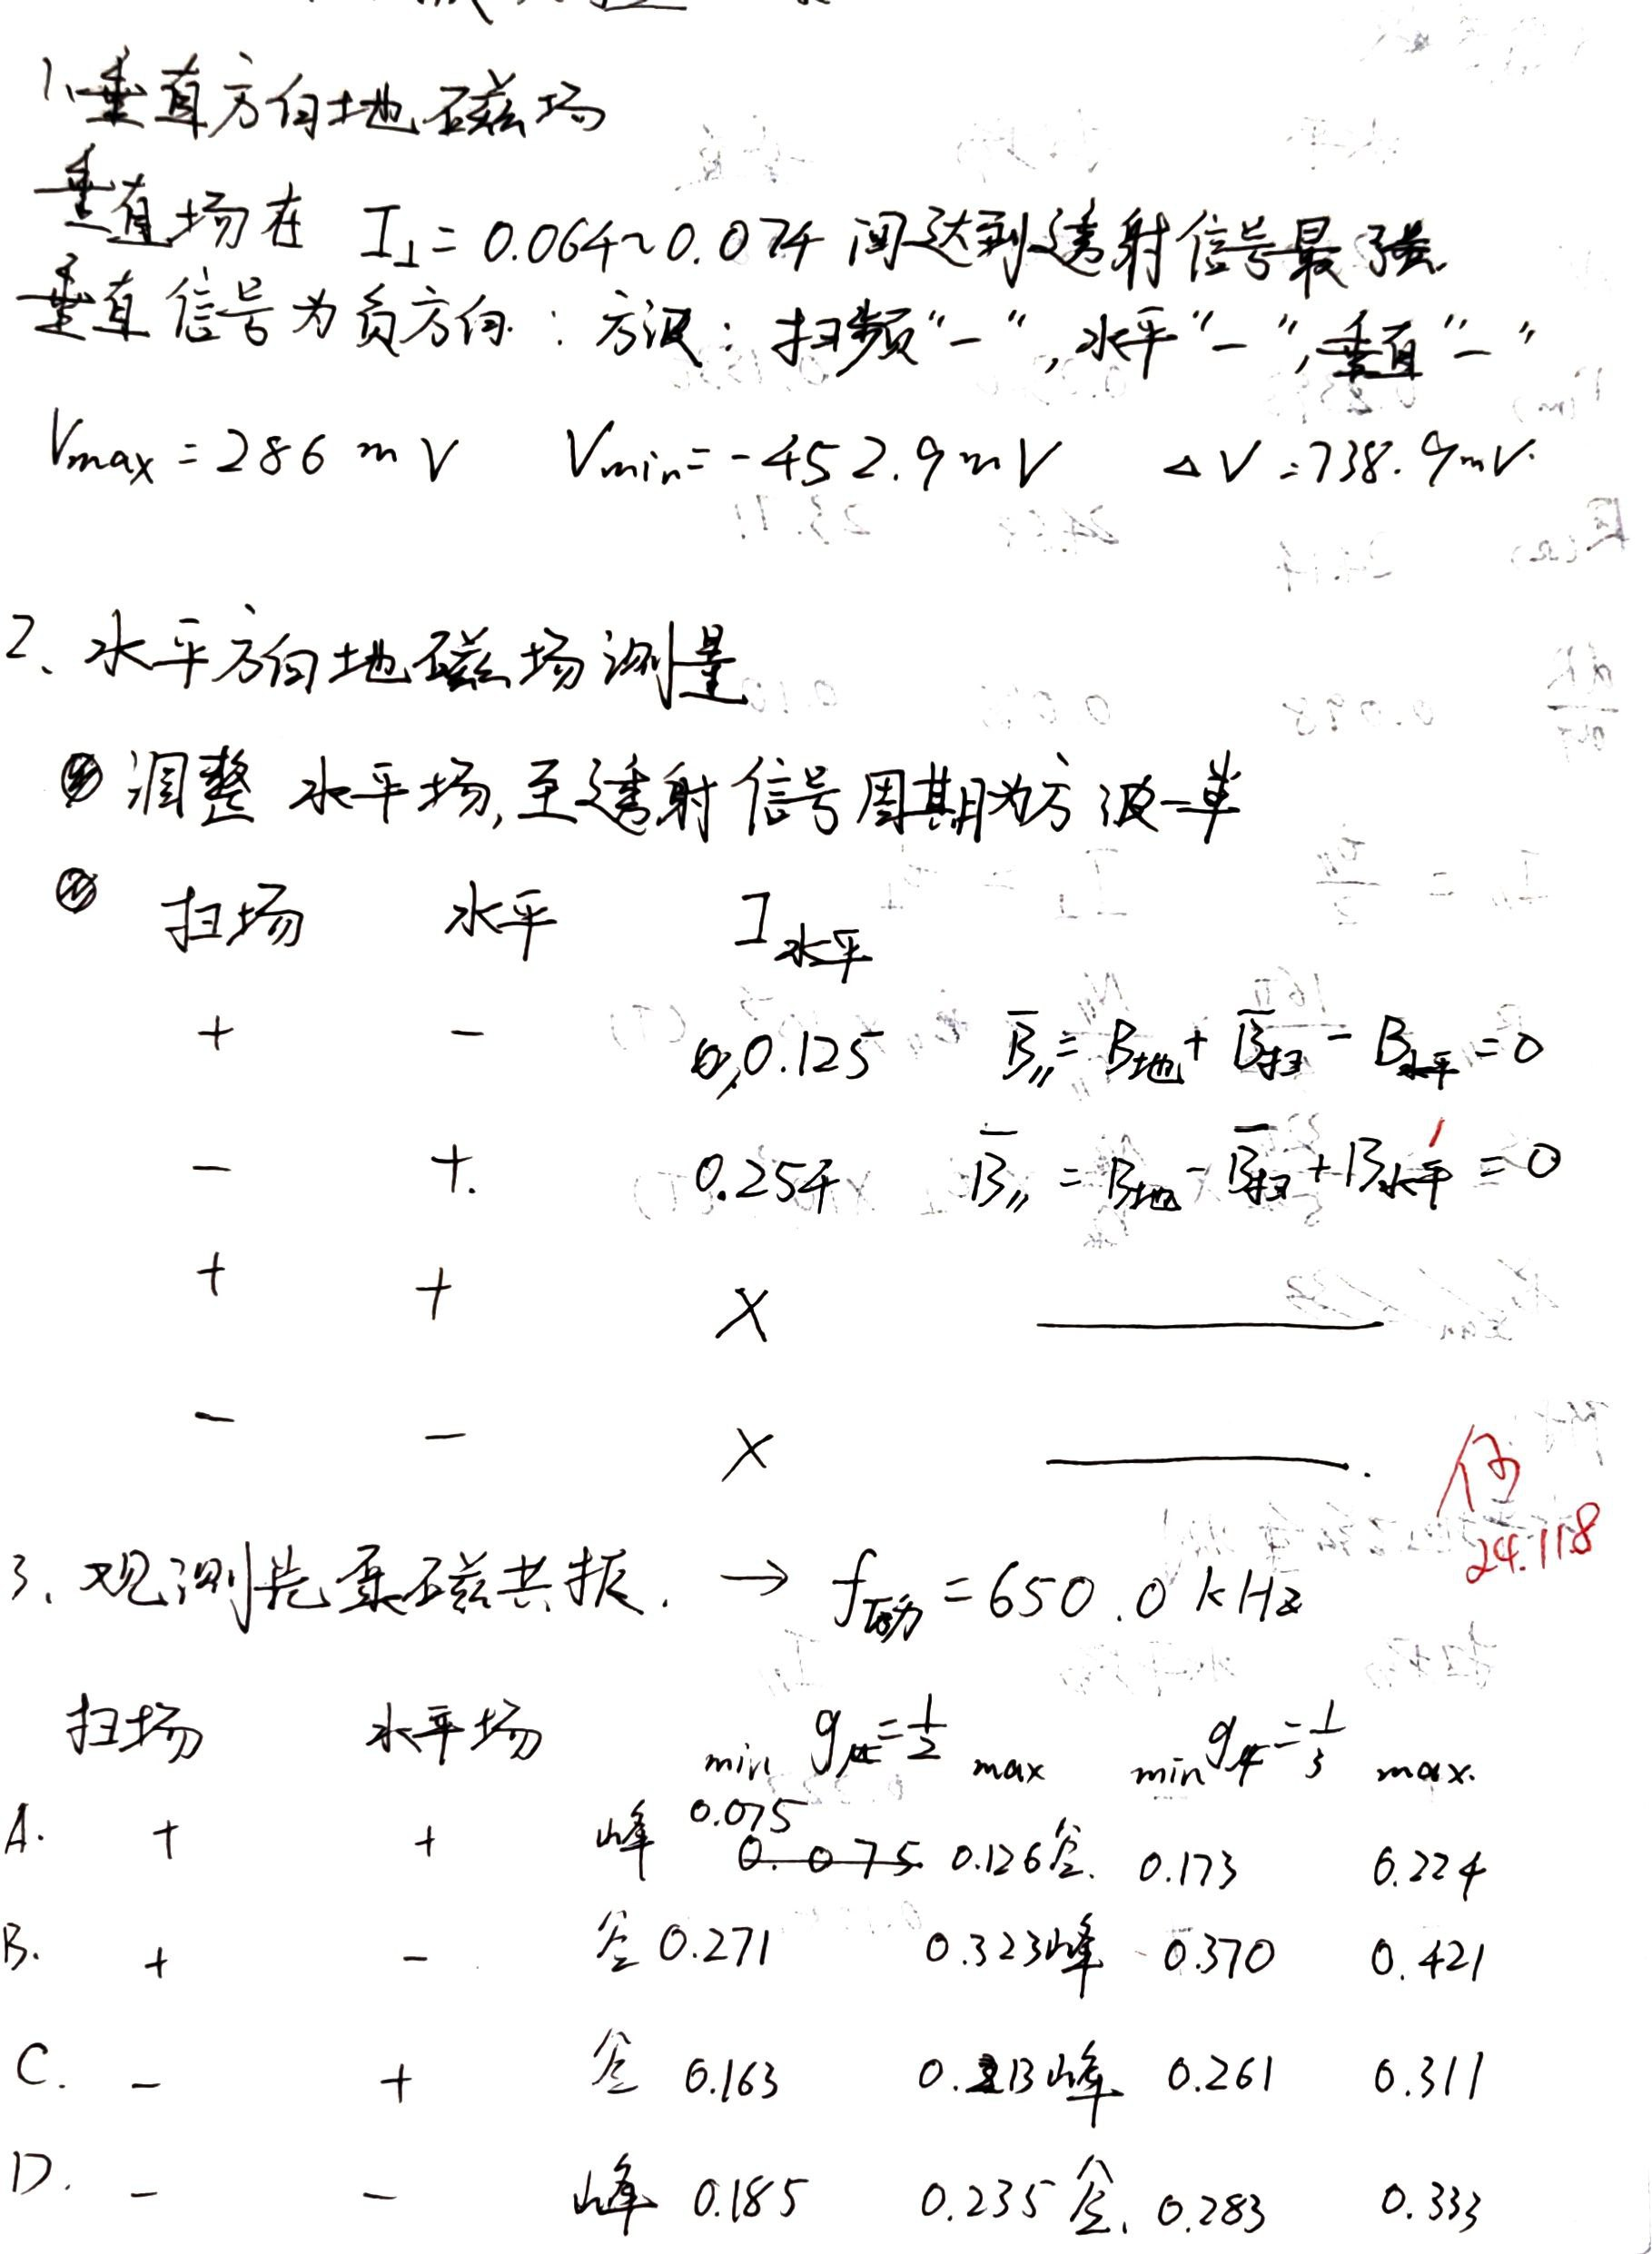
\includegraphics[width=\linewidth]{figures/appedix1.jpg}
        \end{minipage}
        \begin{minipage}[t]{0.49\linewidth}
            \centering
            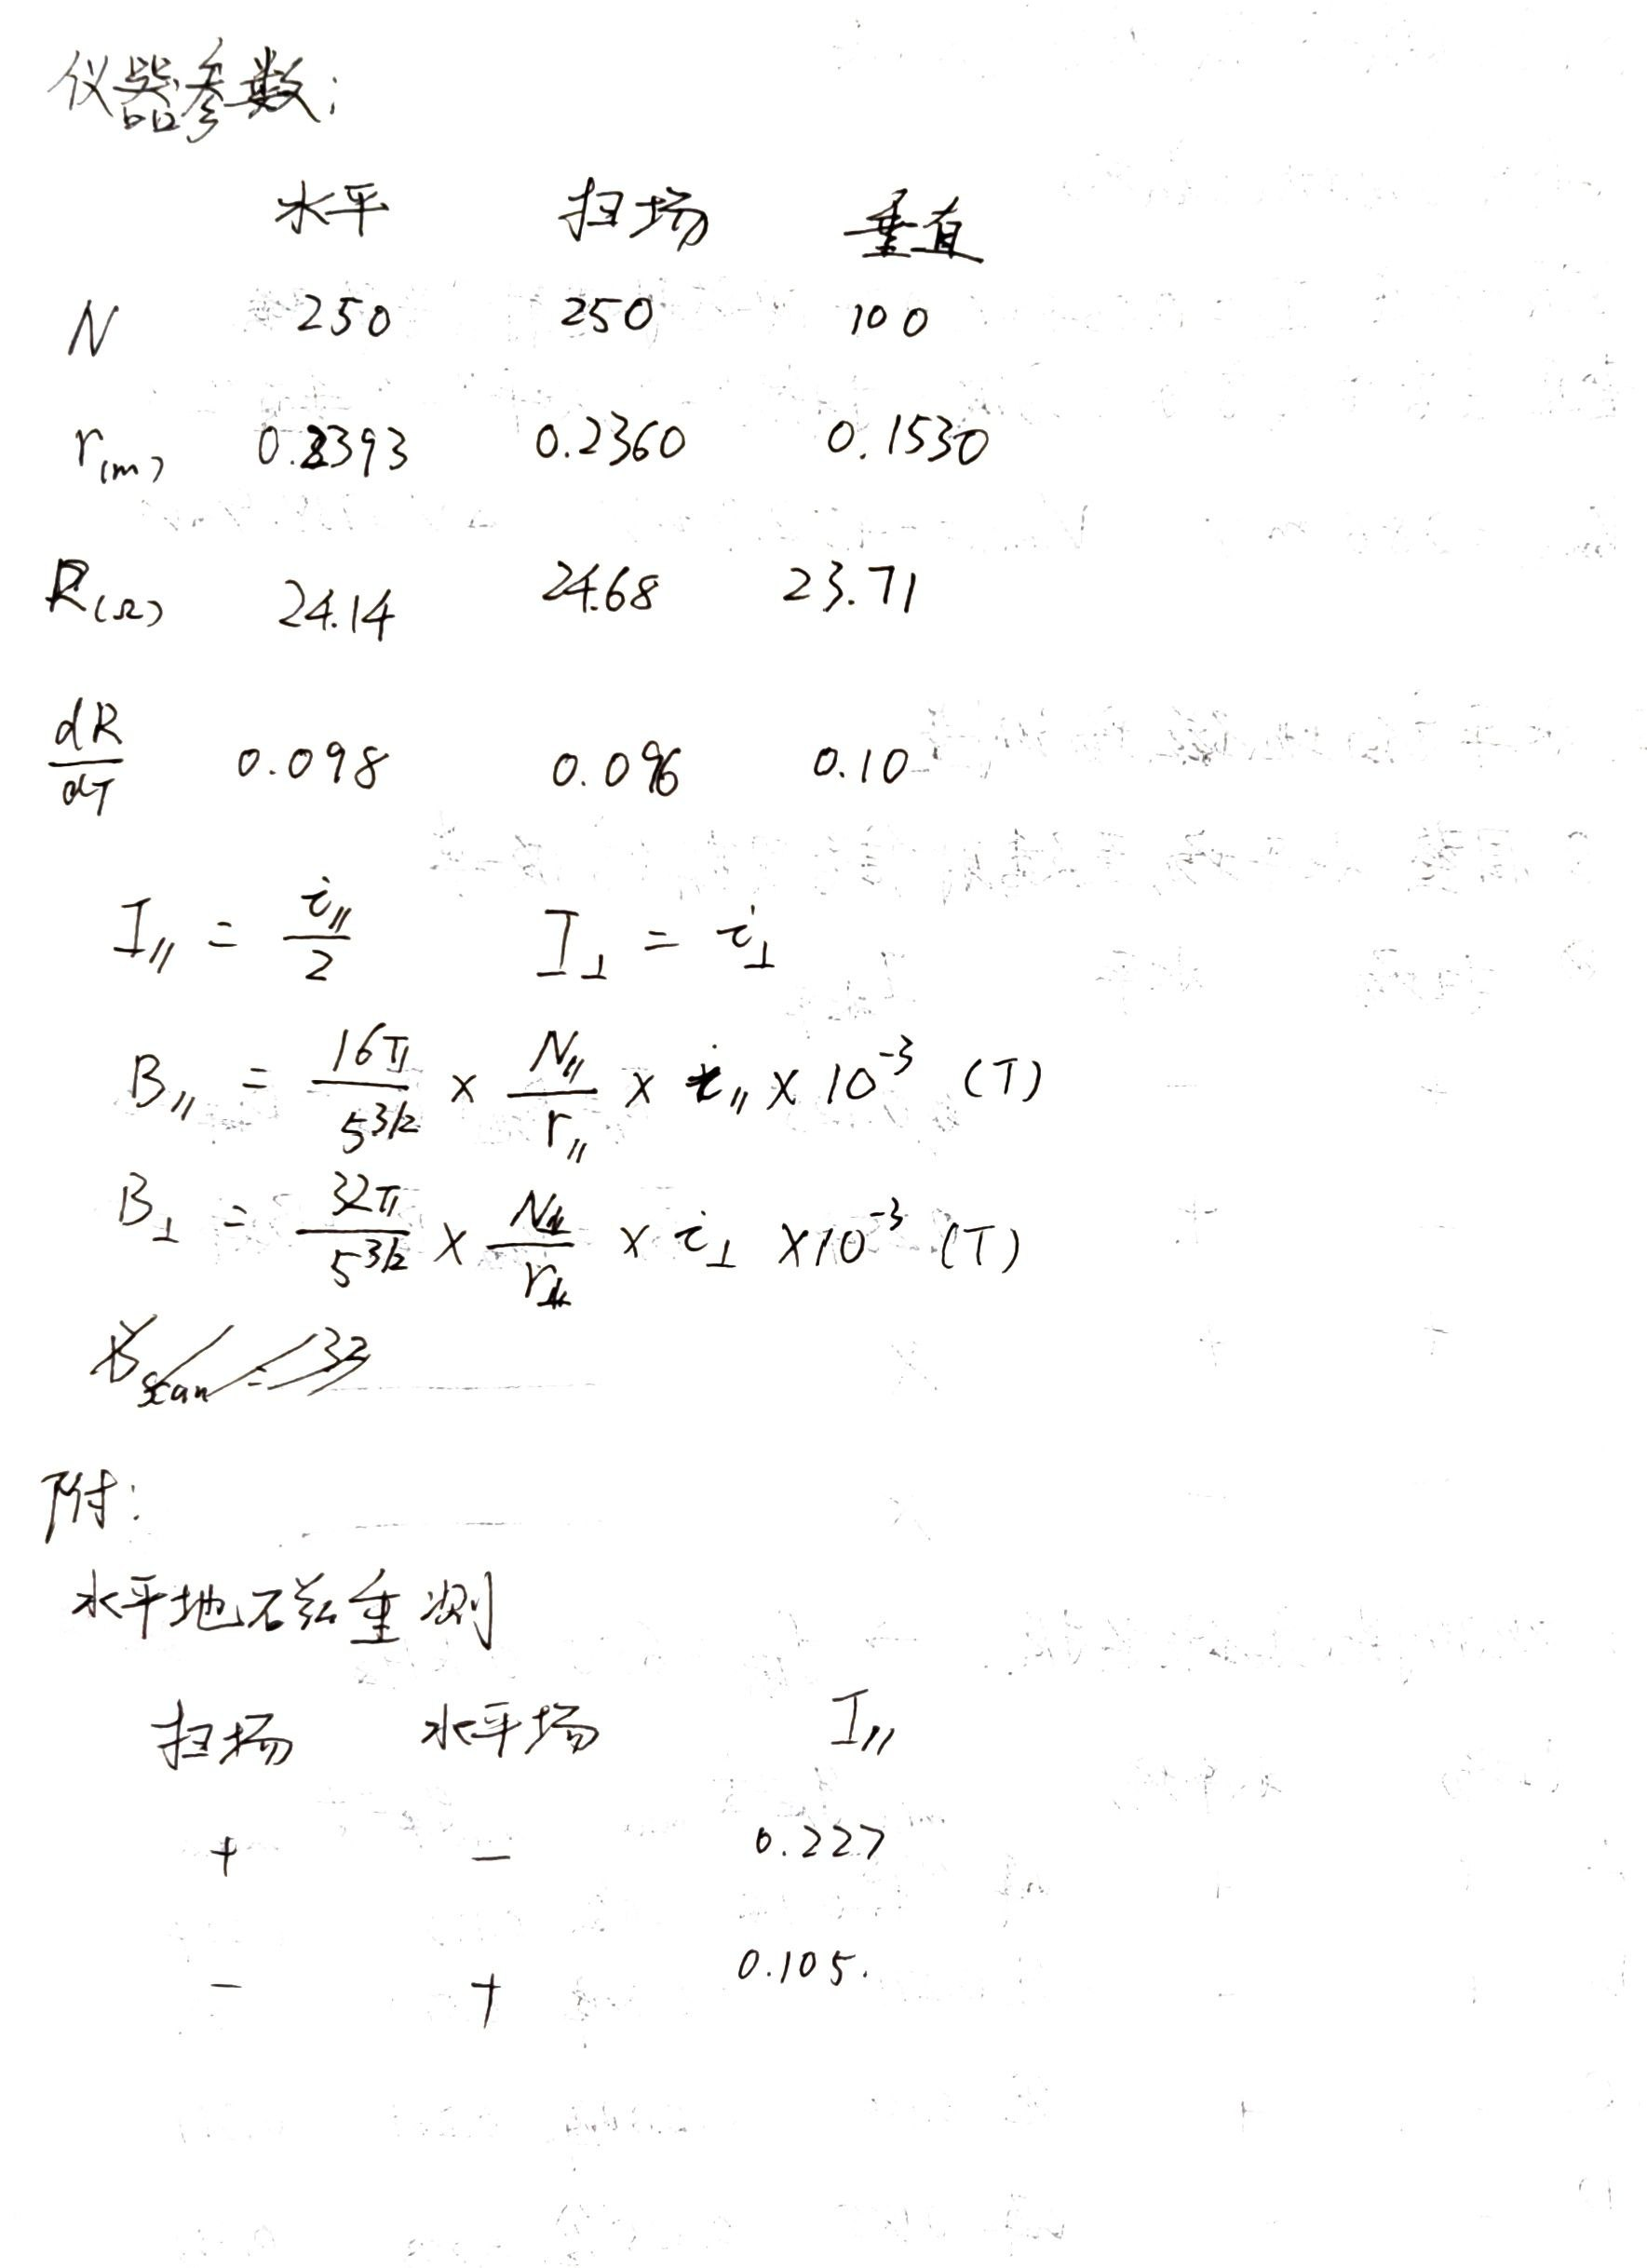
\includegraphics[width=\linewidth]{figures/appedix2.jpg}
        \end{minipage}

        \begin{minipage}[t]{0.49\linewidth}
                \centering
                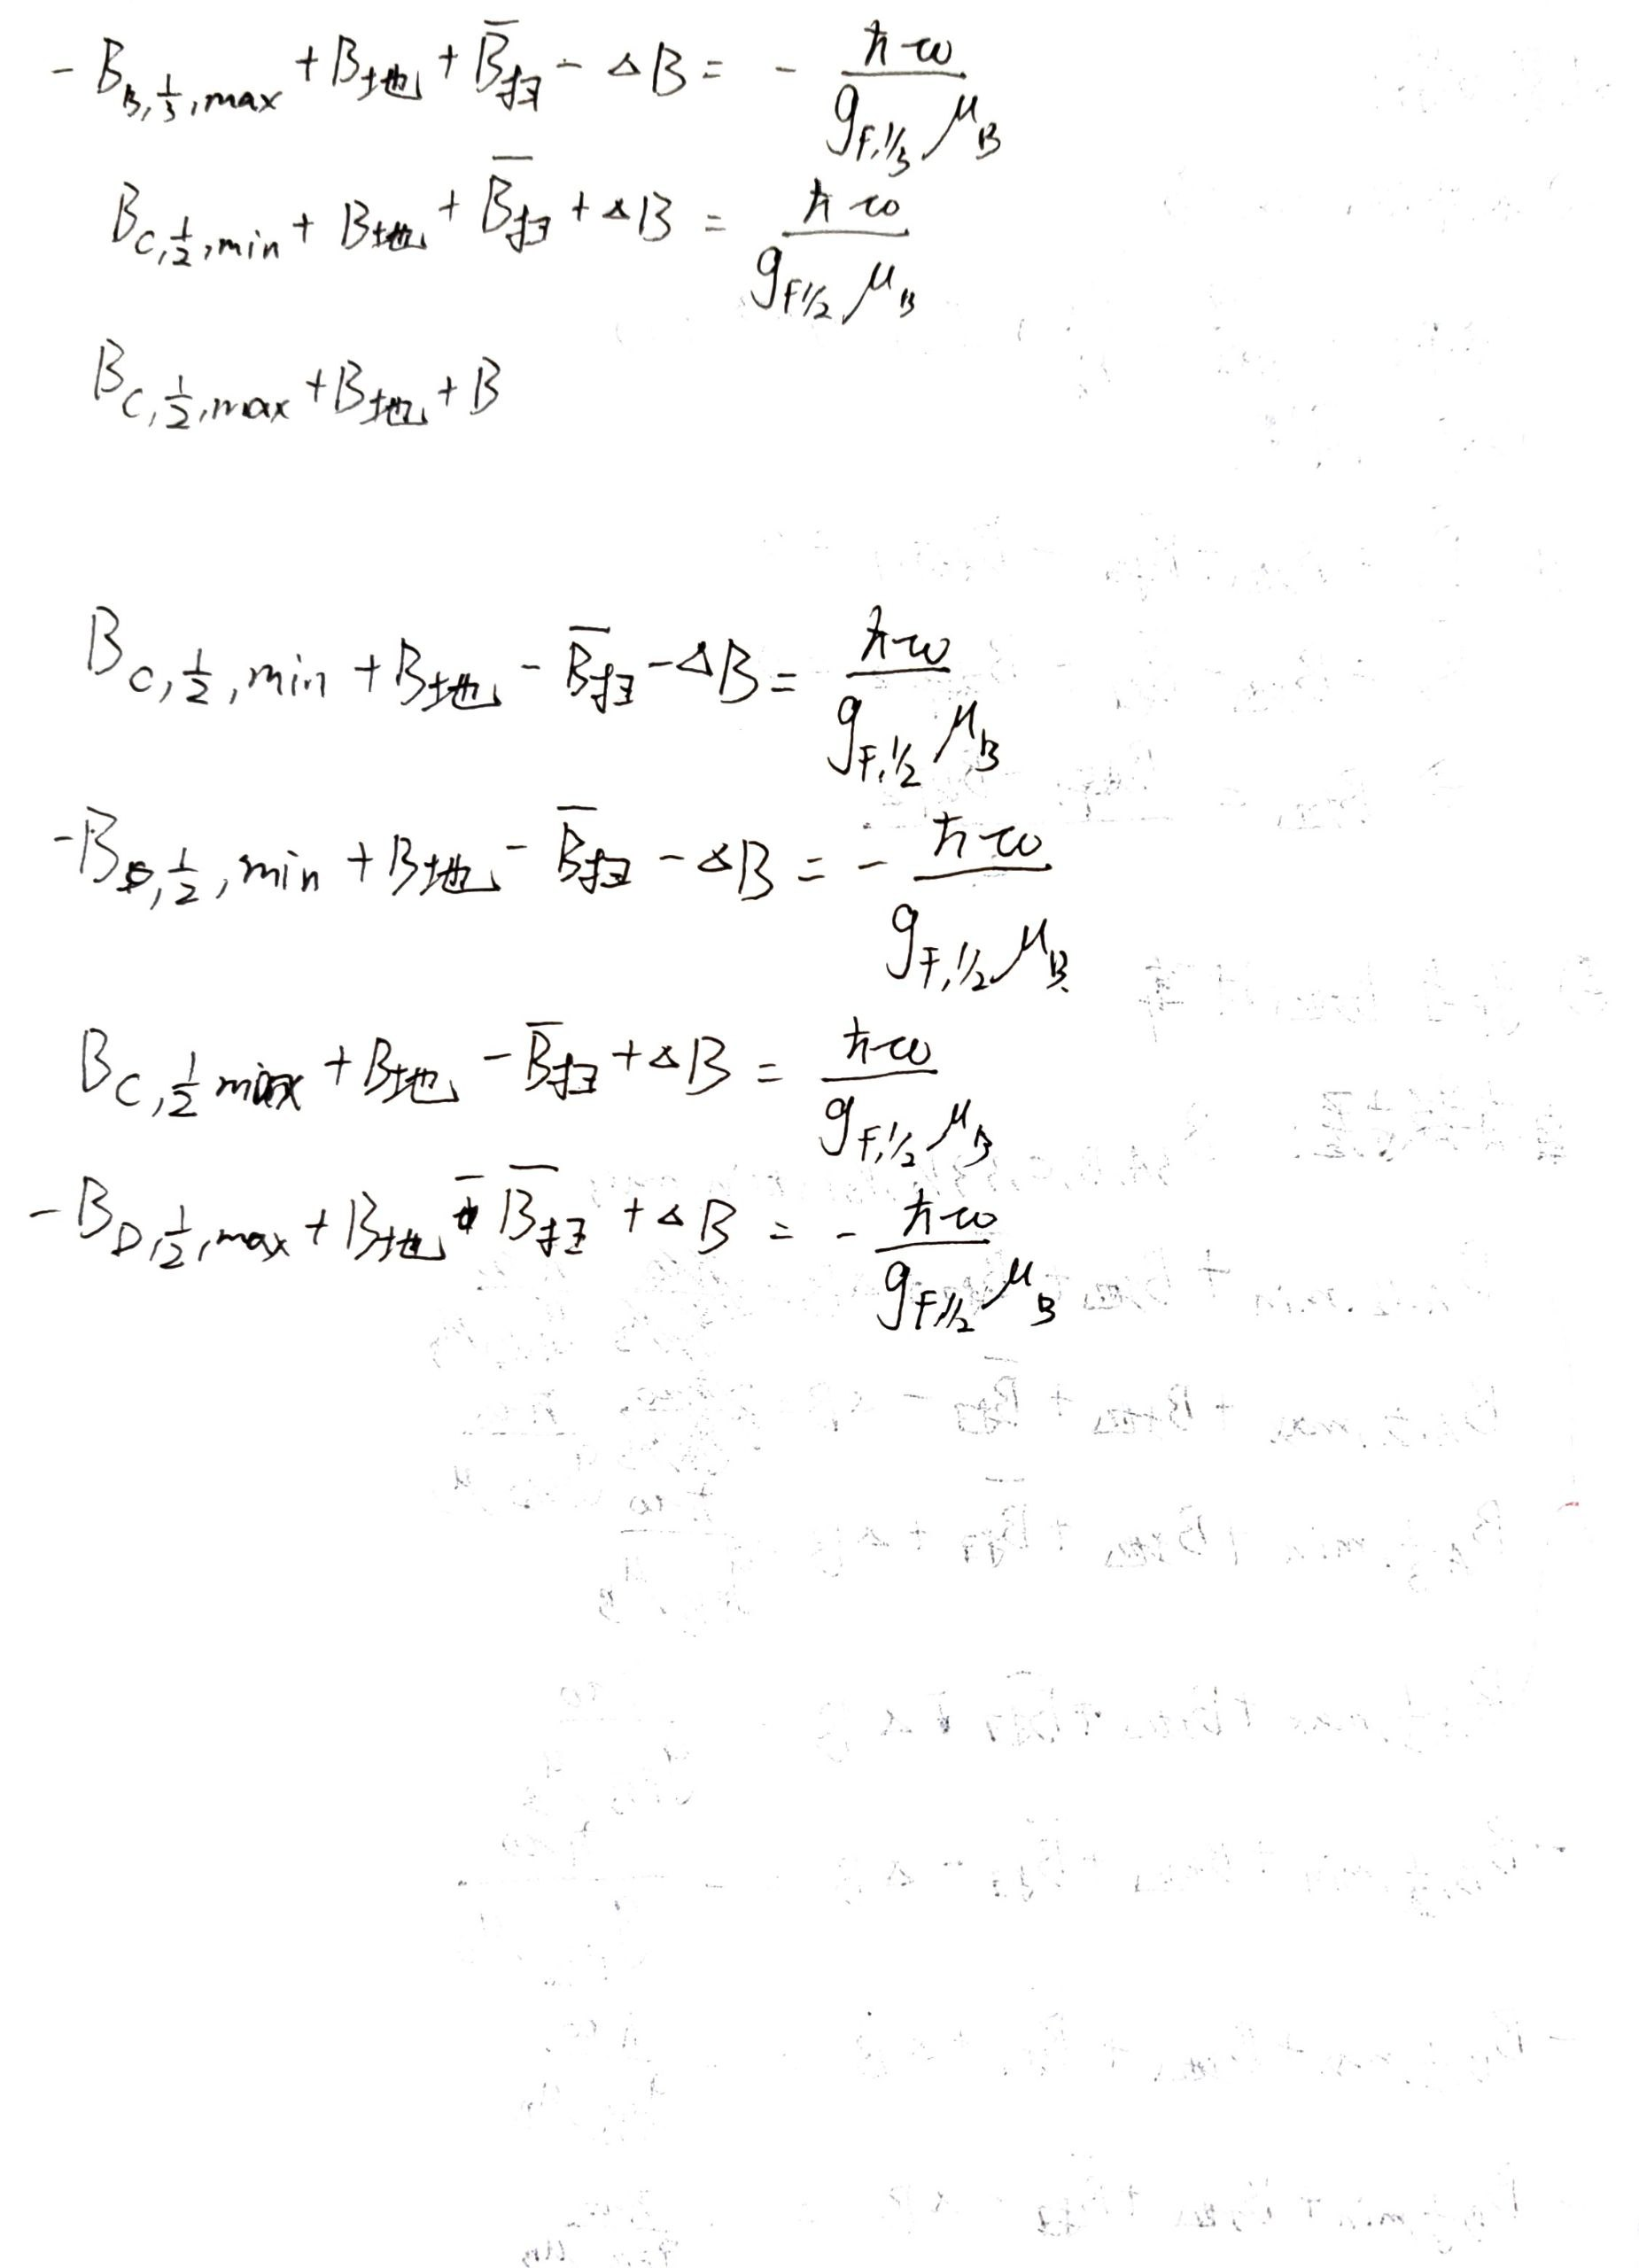
\includegraphics[width=\linewidth]{figures/appedix3.jpg}
        \end{minipage}
        \begin{minipage}[t]{0.49\linewidth}
                \centering
                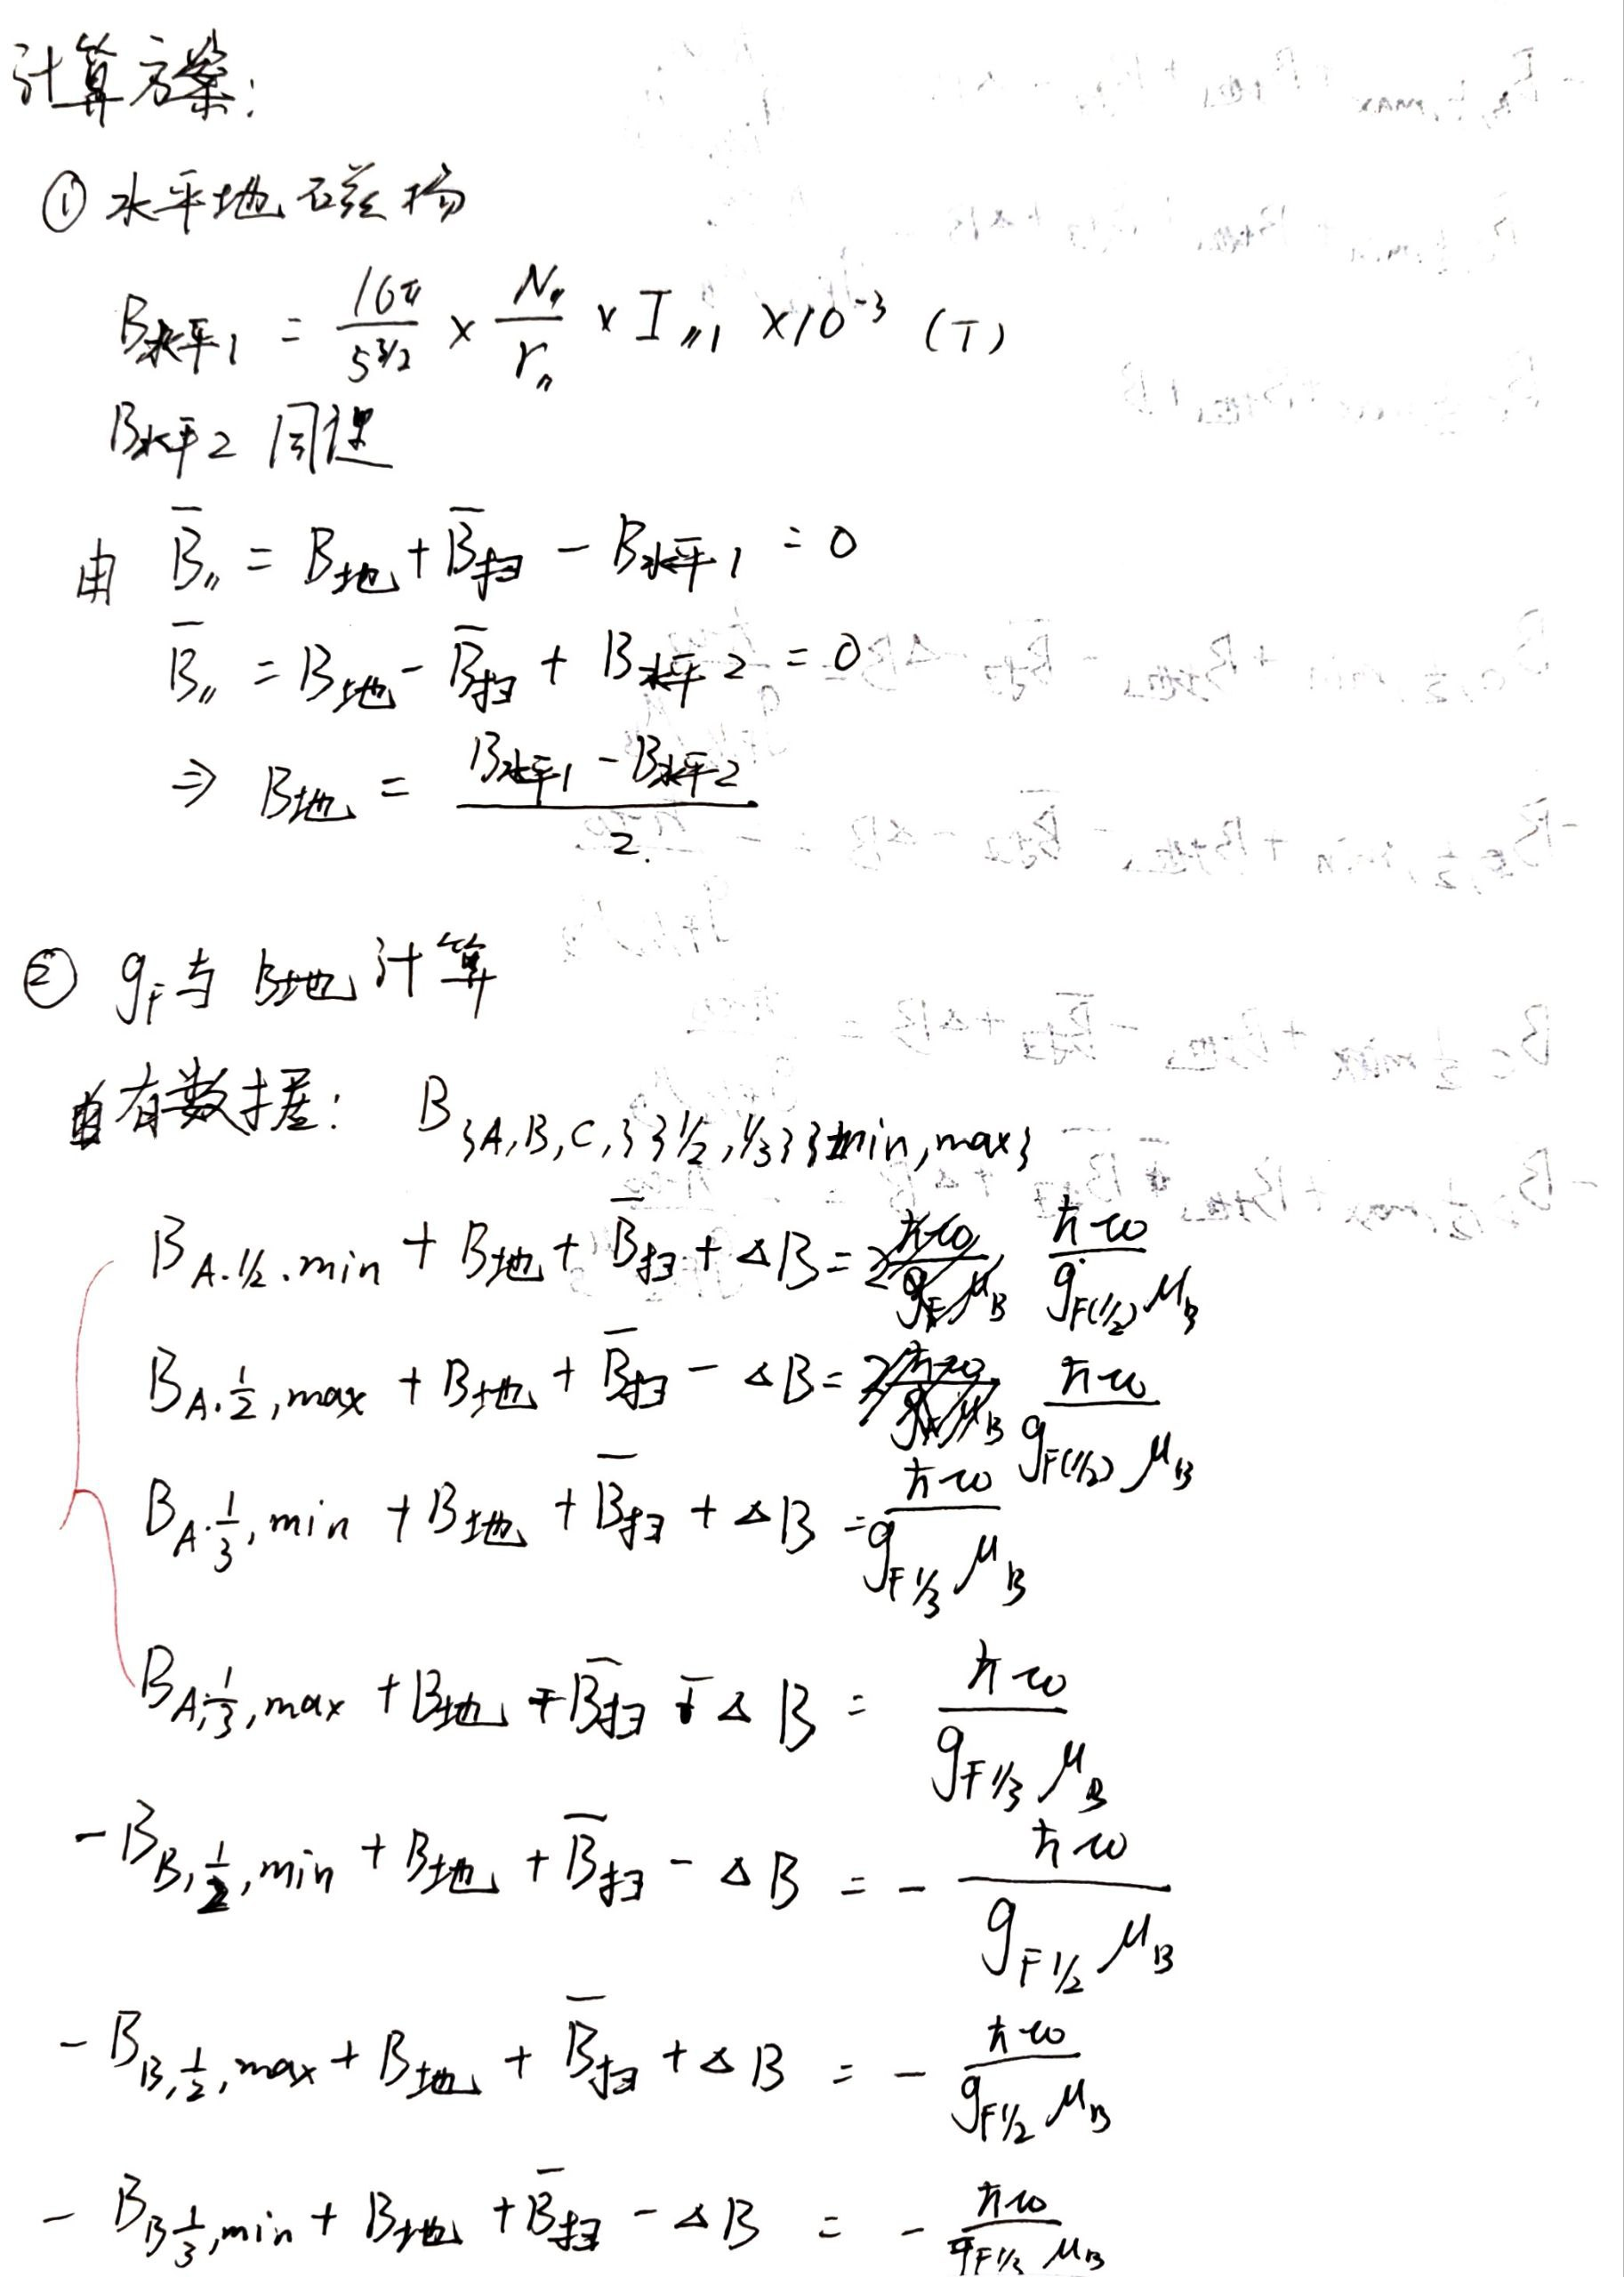
\includegraphics[width=\linewidth]{figures/appedix4.jpg}
        \end{minipage}
        \caption{原始数据}
        \label{fig:image_group}
\end{figure}

\end{document}